\chapter{NumPy}
\label{chp:Numpy}
\epigraph{
	The only thing that remains unsolved is the resolution of the problem.
}{Thomas Wells}

NumPy ist ein Python-Modul mit vielen Einsatzgebieten. Die Dokumentation des Pakets\footnote{\url{https://numpy.org/doc/stable/user/whatisnumpy.html}} wird selbstbewusst eingeleitet mit:
\begin{center}
	\emph{NumPy is the fundamental package for scientific computing in Python.}
\end{center}

Nicht nur werden Routinen für viele häufig auftauchende Aufgaben bereitgestellt; die Umsetzung dieser ist auch bedeutend schneller, als es in \enquote{Vanilla-Python} möglich wäre, da die Kernroutinen in kompilierten C-Libraries vorliegt. Wir erhalten also nicht nur zusätzlichen Komfort, sondern auch einen massiven Speedup bei der Verwendung von NumPy-Funktionen.

\begin{hintbox}[Installation]
Nicht auf allen Systemen ist NumPy sofort vorinstalliert. Um zu testen, ob Ihr System bereits die NumPy-Bibliothek unterstützt, können Sie diesen Code auführen:
\begin{codebox}[Installation von NumPy testen]
\begin{minted}[linenos]{python3}
try:
    import numpy
except ImportError:
    print("numpy is not installed")
else :
    print("numpy is ready for use")
\end{minted}
\end{codebox}

Sollte die Zeile \texttt{numpy is not installed} erscheinen, so können Sie dies einfach nachinstallieren. Rufen Sie hierzu entweder die Anaconda-Konsole auf (Windows, Mac) oder ein reguläres Terminal (Linux). Hier geben Sie die folgende Zeile (Windows, Mac) ein:

\begin{cmdbox}[NumPy Nachinstallieren -- Windows{,} Mac]
\begin{minted}{text}
pip install numpy
\end{minted}
\end{cmdbox}

oder, wenn Sie unter Linux arbeiten:
\begin{cmdbox}[NumPy Nachinstallieren -- Linux]
\begin{minted}{text}
pip3 install numpy
\end{minted}
\end{cmdbox}
\end{hintbox}

Hier kann nur auf die wichtigsten Features eingegangen werden; eine vollständige Referenz finden Sie unter \url{https://numpy.org/doc/stable/numpy-ref.pdf} (1812 Seiten, Stand Juni 2020).

\section{Grundlegendes Objekt}
Für die Arbeit mit NumPy muss natürlich zuerst das Modul geladen werden. Per Konvention geschieht dies mit dem Alias \texttt{np}:
\begin{codebox}[Modul NumPy Laden]
\begin{minted}{python3}
import numpy as np
\end{minted}
\end{codebox}

Auch wenn nicht explizit in allen Code-Beispielen gezeigt, soll in diesem Kapitel immer davon ausgegangen werden, dass dieser \inPy{import} die erste Zeile aller Beispiele sein soll.

Zentrales Objekt in allen NumPy-Anwendungen ist das \emph{Numpy-Array}. In erster Näherung verhält es sich wie eine Ihnen bereits bekannte \inPy{list}: NumPy-Arrays sind Container von geordneten Werten, \ie ein Wert im Container kann durch seinen \emph{Index} eindeutig identifiziert werden. Sie können sowohl eindimensionale als auch mehrdimensionale Objekte darstellen, also beispielsweise Tabellen abbilden. Über NumPy-Arrays kann auch iteriert werden, \ie es ist möglich sie mit einer \inPy{for}-Schleife zu durchlaufen.

Im Gegensatz zu Python-\inPy{list}s müssen aber \emph{alle Einträge} in einem Numpy-Array \emph{denselben Datentyp} haben\footnote{Diese Einschränkung macht die zugründeliegende Speicherstruktur sehr viel einheitlicher und ist mit für den großen Geschwindigkeits-Gewinn verantwortlich, den wir mit NumPy erhalten. In der Praxis schränkt uns dies kaum ein, da wir NumPy ohnehin nur für ähnliche Daten verwenden.}. Bei Tabellen und Tensoren müssen alle Einträge angegeben werden; es ist also nicht möglich, eine Tabelle mit 5 Zeilen in der ersten Spalte und 10 Zeilen in der zweiten Spalte anzulegen.

Erzeugt werden NumPy-Arrays über ihren Konstruktor aus normalen Python-\inPy{list}s\footnote{Genauer: Aus einem \emph{Iterable}. Das bedeutet, dass auch \inPy{tuple}s, ... benutzt werden können, um NumPy-Arrays zu erzeugen.}. Wo versucht wird, die Einschränkungen auf gleichen Datentyp oder ausgefüllte Tabellen zu missachten, wendet NumPy verschiedene Strategien an, um ein kompatibles Objekt zu erzeugen:

\begin{codebox}[Beispiel: NumPy-Arrays erzeugen]
\begin{minted}[linenos]{python3}
import numpy as np

npList   = np.array([1, 2, 3])
npMixed1 = np.array([1, 1.5])
npMixed2 = np.array([1, 1.0, "1.0"])

npTab      = np.array([[1, 2, 3], [4, 5, 6]])
npListList = np.array([[1], [2, 3]])

print(npList)
print(npMixed1)
print(npMixed2)
print(npTab)
print(npListList)
\end{minted}
\end{codebox}

\begin{cmdbox}[Ausgabe: NumPy-Arrays erzeugen]
\begin{minted}{text}
[1 2 3]
[1.  1.5]
['1' '1.0' '1.0']
[[1 2 3]
 [4 5 6]]
[list([1]) list([2, 3])]
\end{minted}
\end{cmdbox}

Wir sehen zunächst, dass die aus \inPy{int}s bestehende \inPy{list [1, 2, 3]} direkt als NumPy-Array übernommen werden kann (erste Zeile der Ausgabe). Für die aus einem \inPy{int} und einem \inPy{float} bestehende \inPy{list [1, 1.5]} rechnet NumPy beide Einträge zu \inPy{float}s um\footnote{Genauer zu \texttt{np.float64}s -- siehe etwas später dazu.}. Die \inPy{list [1, 1.0, "1.0"]} enthält einen String; da nicht jeder String in eine Zahl umgewandelt werden kann, haben die Entwickler von NumPy sich dazu entschieden, dass in so einem Fall \emph{alle Einträge} zu Strings umgewandelt werden.

Im Falle von Tabellen wie der \inPy{list [[1, 2], [3, 4]]} werden die verschachtelten Listen in das interne Schema der NumPy-Bibliothek heruntergebrochen. In diesem Format kann die Tabelle auch \enquote{schön} als Tabelle ausgegeben werden -- ein einziger \inPy{print}-Befehl erzeugt mehrere Zeilen auf dem Bildschirm.

Dagegen ist \inPy{list [[1], [2, 3]]} keine vollständig ausgefüllte Tabelle; NumPy fasst sie daher als Array von \inPy{list}s auf. Die Ausgabe spiegelt genau dies wieder.

\subsection{Datentypen und Attribute des NumPy-Arrays}
Der Speicherbedarf für eine Zahl wird in Python dynamisch angepasst. Für kleine Zahlen werden nur einige wenige Bytes verwendet, größere Zahlen beanspruchen einen langen zusammenhängenden Speicherbereich. Hinzu kommt ein \emph{Descriptor}, also ein Speicherabschnitt, in dem deklariert wird, wie viel Speicherplatz zur Darstellung der Zahl verwendet wird, und wo dieser zu finden ist. Der \inPy{int 4} beansprucht \eg 28 Bytes; für den \inPy{int 2**20} dagegen sind es 32 Bytes und für die Zahl \inPy{2**128} werden 44 Bytes belegt. Diese Flexibilität kommt zum Preis längerer Laufzeiten.

In NumPy hingegen wird für alle Zahlen derselbe Speicherplatz zur Verfügung gestellt, der sich aus dem Datentypen herleitet. Für einen \texttt{np.int64} -- die häufigste Übersetzung für einen Python-\inPy{int} -- werden \emph{immer} 8 Bytes genutzt. Es ist offensichtlich, dass 8 Bytes schneller zu verarbeiten sind als 28. Dafür aber kann es beim Rechnen mit NumPy zu sogenannten \emph{oveverflows} kommen: Das Ergebnis einer Berechnung kann zu groß sein, um im bereitgestellten Speicherbereich abgelegt werden zu können. Tabelle \ref{tab:NumPyDataTypes} enthält eine Übersicht der wichtigsten bereitgestellten Typen. Wie Sie an den aufgelisteten Wertebereichen sehen können, sind die Beschränkungen der Wertebereiche selten von Belang.

Unter \url{https://numpy.org/doc/stable/reference/arrays.dtypes.html} finden Sie weitere Details zum Umgang mit den Numpy-Datentypen.

Im Folgenden wollen wir immer dieselben Arrays in den Beispielen betrachten. Diese seien definiert durch:
\begin{codebox}[Beispiel: Ausgangsarrays für die folgenden Beispiele]
\begin{minted}[linenos]{python3}
import numpy as np
import math

npList = np.array([1, 2, 3])
npTab  = np.array([[1.1, 2.2, 3.3], [4.4, 5.5, 6.6]])
\end{minted}
\end{codebox}

\begin{figure}[h]  % abuse of the figure environment to make it a float... define a floating tcolorbox at some point...
\begin{tcolorbox}[title=Übliche NumPy-Datentypen]
\begin{center}
\rowcolors{1}{}{tabcontrast}
\begin{tabular}{lm{.15\linewidth}m{.3\linewidth}m{.25\linewidth}}
	\textbf{NumPy-Typ}     & \textbf{Beschreibung} & \textbf{Wertebereich} & \textbf{Entsprechung in C-Artigen Sprachen} \tabcrlf
	\texttt{np.int8}       & Ganzzahl & -128 bis +127                                                                            & \texttt{char} \\
	\texttt{np.int16}      & Ganzzahl & -32\,768 bis +32\,767                                                                    & \texttt{short} \\
	\texttt{np.int32}      & Ganzzahl & -2\,147\,483\,648 bis +2\,147\,483\,647                                                  & \texttt{long} \\
	\texttt{np.int64}      & Ganzzahl & -9\,223\,372\,036\,854\,775\,808 bis +9\,223\,372\,036\,854\,775\,807                    & \texttt{long long} \\
	\texttt{np.uint8}      & Ganzzahl & 0 bis +255                                                                               & \texttt{unsigned char} \\
	\texttt{np.unit16}     & Ganzzahl & 0 bis +65\,536                                                                           & \texttt{unsigned short} \\
	\texttt{np.unit32}     & Ganzzahl & 0 bis +4\,294\,967\,295                                                                  & \texttt{unsigned long} \\
	\texttt{np.unit64}     & Ganzzahl & 0 bis +18\,446\,744\,073\,709\,551\,615                                                  & \texttt{unsigned long long}\\
	\texttt{np.float32}    & Fließkommazahl & ca. $-3.4 \times 10^{38}$ bis $+3.4 \times 10^{38}$, ca. 7 signifikante Ziffern    & \texttt{float} \\
	\texttt{np.float64}    & Fließkommazahl & ca. $-1.7 \times 10^{308}$ bis $+1.7 \times 10^{308}$, ca. 15 signifikante Ziffern & \texttt{double}\\
	\texttt{np.complex64}  & Komplexe Zahl & Real und Imaginärteil jeweils wie \texttt{np.float32}                               & \texttt{float complex} \\
	\texttt{np.complex128} & Komplexe Zahl & Real und Imaginärteil jeweils wie \texttt{np.float64}                               & \texttt{double complex}  \\
\end{tabular}
\captionof{table}{Datentypen in NumPy}
\label{tab:NumPyDataTypes}
Siehe auch {https://numpy.org/doc/stable/user/basics.types.html} für weitere Details.
\end{center}
\end{tcolorbox}
\end{figure}

Der Datentyp der Elemente eines NumPy-Arrays kann über das Attribut \texttt{dtype} abgefragt werden:
\begin{tcbraster}[raster columns=2,
                  raster equal height,
                  nobeforeafter,
                  raster column skip=0.5cm]
\begin{codebox}[Beispiel: Zugrundeliegender Datentyp]
\begin{minted}[linenos, firstnumber=5]{python3}
# ...
print(npList.dtype)
print(npTab.dtype)
\end{minted}
\end{codebox}
%
\begin{cmdbox}[Ausgabe: Zugrundeliegender Datentyp]
\begin{minted}{text}
int64
float64
\end{minted}
\end{cmdbox}
\end{tcbraster}

Ebenso wie der Datentyp kann auch die \emph{Form} eines NumPy-Arrays mit \texttt{shape} abgefragt werden. Die \enquote{Antwort} ist en \inPy{tuple} mit der Zahl der Elemente in jeder Dimension:

\begin{tcbraster}[raster columns=2,
                  raster equal height,
                  nobeforeafter,
                  raster column skip=0.5cm]
\begin{codebox}[Beispiel: Form eines NumPy-Arrays]
\begin{minted}[linenos, firstnumber=8]{python3}
# ...
print(npList.shape)
print(npTab.shape)
\end{minted}
\end{codebox}
%
\begin{cmdbox}[Ausgabe: Form eines NumPy-Arrays]
\begin{minted}{text}
(3,)
(2, 3)
\end{minted}
\end{cmdbox}
\end{tcbraster}

Die \emph{Gesamtzahl der Elemente} in einem NumPy-Array und die \emph{Gesamtzahl der Dimensionen} sind in den \inPy{int}-Attributen \texttt{size} und \texttt{ndim} gespeichert. Alternativ könnte man diese Informationen auch aus \texttt{shape} gewinnen:

\begin{codebox}[Beispiel: Anzahl Elemente \& Dimensionen, width=.57\linewidth, nobeforeafter, equal height group = grpXmpSimpleNDimsElements]
\begin{minted}[linenos, firstnumber=11]{python3}
# ...
print(npList.size, math.prod(npList.shape))
print(npTab .size, math.prod(npTab.shape))
print()
print(npList.ndim, len(npList.shape))
print(npTab .ndim, len(npTab.shape))
\end{minted}
\end{codebox}
%
\hspace{0.5cm}
\begin{cmdbox}[Anzahl Elemente \& Dimensionen, width=.4\linewidth, nobeforeafter, equal height group = grpXmpSimpleNDimsElements]
\begin{minted}{text}
3 3
12 12

1 1
2 2
\end{minted}
\end{cmdbox}

Schließlich kann für die Anbindung an C-Bibliotheken auch die Speicheradresse in Erfahrung gebracht werden, wo die Daten des NumPy-Arrays abgelegt sind. Hierzu dient das Attribut \texttt{data}. Der Rückgabewert ist ein \texttt{MemoryView}-Objekt, das an dieser Stelle nicht näher besprochen werden soll.

\begin{codebox}[Beispiel: Adresse eines Arrays, width=.57\linewidth, nobeforeafter, equal height group = grpXmpNumPyMemory]
\begin{minted}[linenos, firstnumber=17]{python3}
# ...
print(npList.data)
\end{minted}
\end{codebox}
%
\hspace{0.5cm}
\begin{cmdbox}[Ausgabe: Adresse eines Arrays, width=.4\linewidth, nobeforeafter, equal height group = grpXmpNumPyMemory]
\begin{minted}{text}
<memory at 0x7fa439743b80>
\end{minted}
\end{cmdbox}

Bei komplexwertigen Arrays kann der Real- und Imaginärteil für alle Elemente als eigenes Array über die Attribute \texttt{real} und \texttt{imag} abgegriffen werden.

\section{Indices und NumPy-Arrays}
NumPy-Arrays können genauso indiziert werden wie Python-\inPy{list}s. Im Gegensatz zu diesen bietet NumPy aber einigen zusätzlichen Komfort.

Bei mehrdimensionalen Listen kann ein einzelnes Element angesprochen werden, indem ein \inPy{tuple} mit seinen Koordinaten übergeben wird. Für das NumPy-Array \texttt{a} ist also der Zugriff \texttt{a[i, j]} gleichbedeutend mit dem Zugriff \texttt{a[i][j]}. Ersteres dürfte den meisten ProgrammiererInnen als leichter zu Tippen und zu Lesen erscheinen.

Wie Python-\inPy{list}s unterstützen auch NumPy-Arrays Slicing. Dies kann auch mit der Multi-Index-Schreibweise kombiniert werden, \ie Slices können durch Kommata voneinander getrennt werden, um einen Unter-Block des NumPy-Arrays anzugeben
\begin{codebox}[Beispiel: Einfache Index-Zugriffe]
\begin{minted}[linenos]{python3}
npTab = np.array(
    [[ 1,  2,  3],
     [ 4,  5,  6],
     [ 7,  8,  9],
     [10, 11, 12]]
)

print("entire table:\n", npTab)
print()
print("element (0, 1):", npTab[0, 1])
print("last row:", npTab[-1])
print("column 1:", npTab[:,1])
print("upper left square:\n", npTab[0:2, 0:2])
\end{minted}
\end{codebox}

\begin{cmdbox}[Ausgabe: Einfache Index-Zugriffe]
\begin{minted}{text}
entire table:
 [[ 1  2  3]
 [ 4  5  6]
 [ 7  8  9]
 [10 11 12]]

element (0, 1): 2
last row: [10 11 12]
column 1: [ 2  5  8 11]
upper left square:
 [[1 2]
 [4 5]]
\end{minted}
\end{cmdbox}

Weiter kann auch ein NumPy-Array oder eine Python-\inPy{list} oder ein NumPy-Array als Index-Liste übergeben werden. Jedes Element des NumPy-Arrays wird dann als Index behandelt. Hat das Index-Array mehrere Dimensionen, so wird für jede Dimension eine eigene Ergebnis-Liste angelegt:

\begin{tcbraster}[raster columns=2,
                  raster equal height,
                  nobeforeafter,
                  raster column skip=0.5cm]
\begin{codebox}[Beispiel: Zugriffe mit Index-Arrays]
\begin{minted}[linenos, firstnumber=14]{python3}
# ...

npIdcs = np.array([1, -1])
print(npTab[npIdcs])

npTup = np.array([[1, 2], [2, 1]])
print(npTab[npTup])
\end{minted}
\end{codebox}
%
\begin{cmdbox}[Ausgabe: Zugriffe mit Index-Arrays]
\begin{minted}{text}
[[ 4  5  6]
 [10 11 12]]
[[[4 5 6]
  [7 8 9]]

 [[7 8 9]
  [4 5 6]]]
\end{minted}
\end{cmdbox}
\end{tcbraster}

Das Index-Array darf auch aus \inPy{bool}s bestehen. In diesem Fall müssen Index-Array und des NumPy-Array dieselbe Länge haben. Zurückgemeldet werden diejenigen Elemente des NumPy-Arrays, für die im Index-Array \inPy{True} eingetragen war. Man spricht auch von Indexmasken:

\begin{tcbraster}[raster columns=2,
                  raster equal height,
                  nobeforeafter,
                  raster column skip=0.5cm]
\begin{codebox}[Beispiel: Indexmasken]
\begin{minted}[linenos, firstnumber=22]{python3}
# ...
mask = [True, False, False, True]
print(npTab[mask])
\end{minted}
\end{codebox}
%
\begin{cmdbox}[Ausgabe: Indexmasken]
\begin{minted}{text}
[[ 1  2  3]
 [10 11 12]]
\end{minted}
\end{cmdbox}
\end{tcbraster}

Ein spezieller Index ist der Wert \texttt{np.newaxis}: Mit diesem kann eine neue Dimension in ein NumPy-Array eingeführt werden:

\begin{codebox}[Beispiel: Neue Dimension Einführen]
\begin{minted}[linenos, firstnumber=25]{python3}
# ...

print( npList[np.newaxis] )
print( npList )
print()
print( npTab[np.newaxis] )
print( npTab[:,np.newaxis] )
\end{minted}
\end{codebox}
%
\begin{cmdbox}[Ausgabe: Neue Dimension Einführen]
\begin{minted}{text}
[[1 2 3]]
[1 2 3]

[[[ 1  2  3]
  [ 4  5  6]
  [ 7  8  9]
  [10 11 12]]]
[[[ 1  2  3]]

 [[ 4  5  6]]

 [[ 7  8  9]]

 [[10 11 12]]]
\end{minted}
\end{cmdbox}

Ausgehend von der eindimensionalen \texttt{npList} erzeugt \texttt{npList[np.newaxis]} also ein zweidimensionales Objekt, also eine Tabelle mit einer Zeile und drei Spalten. Dieses Objekt wird neu erzeugt, \ie das originale Objekt \texttt{npList} wird also nicht verändert. Bei mehrdimensionalen Objekten gibt die Position von \texttt{np.newaxis} in der Index-Liste an, \enquote{in welche Richtung} die neue Dimension eingefügt wird. So ist \texttt{npTab[np.newaxis]} ein 1x4x3-Tensor und kann als \enquote{Liste von 4x3-Tabellen mit einem Eintrag} interpretiert werden; dagegen ist \texttt{npTab[:,np.newaxis]} ein 4x1x3-Tensor und kann als \enquote{Liste von 1x3-Tabellen mit vier Einträgen} interpretiert werden.

\section{Methoden zum schnellen Erstellen von NumPy-Arrays}
Bestimmte Formen von Arrays kehren immer wieder. Die wichtigsten davon seien hier zusammengefasst. Siehe auch \url{https://numpy.org/doc/stable/reference/routines.array-creation.html} für eine ausführliche Liste.

\subsection{Gleichmäßig ansteigende Folgen}
Von Python kennen wir bereits den Befehl \inPy{range}, der Folgen von \inPy{int}s erzeugt. NumPy erlaubt, auch Arrays anderer Datentypen zu erzeugen.

Die direkte Entsprechung von \inPy{range} ist der Befehl \texttt{arange}: Er kann entweder in der Form \texttt{np.arange(Start, Stop, Schrittweite)} oder \texttt{np.arange(Stop)} benutzt werden, und erzeugt ein NumPy-Array, das die Werte von \texttt{Start} bis ausschließlich \texttt{Stop} enthält. Im Falle der zweiten Syntax werden die Zahlen von \inPy{0} bis ausschließlich \texttt{Stop} in Abständen von \inPy{1} erzeugt, wie bei \inPy{range}. Anders als dort ist die Ausgabe aber kein Generator-Objekt, sondern ein NumPy-Array. Außerdem darf \texttt{Schrittweite} auch eine Nicht-Ganzzahl sein. Das Optionale Argument \texttt{dtype} kann außerdem dazu genutzt werden, um den Datentyp der Array-Elemente festzulegen:

\begin{codebox}[Beispiel: \texttt{arange}]
\begin{minted}[linenos]{python3}
arr1 = np.arange(5)
arr2 = np.arange(5, 10, dtype=np.float64)
arr3 = np.arange(0, 2, 0.25)
\end{minted}
\end{codebox}
%
\begin{codebox}[]
\begin{minted}[linenos, firstnumber=last]{python3}
print(arr1.dtype, arr1, sep='\t')
print(arr2.dtype, arr2, sep='\t')
print(arr3.dtype, arr3, sep='\t')
\end{minted}
\end{codebox}

\begin{cmdbox}[Ausgabe: \texttt{arange}]
\begin{minted}{text}
int64   [0 1 2 3 4]
float64 [5. 6. 7. 8. 9.]
float64 [0.   0.25 0.5  0.75 1.   1.25 1.5  1.75]
\end{minted}
\end{cmdbox}

Ganz ähnlich arbeitet \texttt{linspace}. Im Gegensatz zur Schrittweite wird hier jedoch die \emph{Anzahl der Elemente im Array} angegeben. Lässt man diese Angabe aus, geht NumPy automatisch von 50 Array-Elementen aus. Außerdem wird der Wert \texttt{Stop} hier \emph{mit eingeschlossen}. Ein \texttt{Start}-Wert \emph{muss} angegeben werden. Auch hier kann der optionale Parameter \texttt{dtype} angegeben werden. Standard-Typ ist \texttt{np.float64}.

\begin{codebox}[Beispiel: \texttt{linspace}]
\begin{minted}[linenos]{python3}
arr1 = np.linspace(0, 4.90)
arr2 = np.linspace(0, 2, 11)

print(arr1.dtype, arr1, sep='\t')
print(arr2.dtype, arr2, sep='\t')
\end{minted}
\end{codebox}

\begin{cmdbox}[Ausgabe: \texttt{linspace}]
\begin{minted}{text}
float64 [0.  0.1 0.2 0.3 0.4 0.5 0.6 0.7 0.8 0.9 1.  1.1 1.2 1.3 1.4 1.5 1.6 1.7
 1.8 1.9 2.  2.1 2.2 2.3 2.4 2.5 2.6 2.7 2.8 2.9 3.  3.1 3.2 3.3 3.4 3.5
 3.6 3.7 3.8 3.9 4.  4.1 4.2 4.3 4.4 4.5 4.6 4.7 4.8 4.9]
float64 [0.  0.2 0.4 0.6 0.8 1.  1.2 1.4 1.6 1.8 2. ]
\end{minted}
\end{cmdbox}

In manchen Situationen braucht man keine Werte, die durch einen konstanten Abstand gegeben sind, sondern durch einen konstanten Faktor. Zwischen einem Element \texttt{a[i]} und \texttt{a[i + 1]} soll also immer die Beziehung \texttt{a[i + 1] = factor * a[i]} gelten. Dies wird sehr leicht über die Befehle \texttt{geomspace} und \texttt{logspace} erreicht.

Wie auch bei \texttt{linspace} werden bei \texttt{geomspace} die Werte \texttt{Start}, \texttt{Stop} und \texttt{Anzahl} angegeben. Bei Auslassen von \texttt{Anzahl} geht NumPy auch wieder von \inPy{50} aus. Auch hier kann der optionale Parameter \texttt{dtype} angegeben werden.

\begin{codebox}[Beispiel: \texttt{geomspace}]
\begin{minted}[linenos]{python3}
arr = np.geomspace(2, 1024, 10)
print(arr.dtype, arr)
\end{minted}
\end{codebox}

\begin{cmdbox}[Ausgabe: \texttt{geomspace}]
\begin{minted}{text}
float64 [   2.    4.    8.   16.   32.   64.  128.  256.  512. 1024.]
\end{minted}
\end{cmdbox}

Der Befehl \texttt{logspace} arbeitet nach demselben Schema wie \texttt{geomspace}; Angegeben werden jedoch nicht der Start- und Stop\emph{wert}, sondern die \emph{Exponenten} sowie die Basis \texttt{base} mit dem Default-Wert \inPy{10.0}. Zu den Parametern gehören auch wieder \texttt{Anzahl=50} und \texttt{dtype=np.float64}

\begin{codebox}[Beispiel: \texttt{logspace}]
\begin{minted}[linenos]{python3}
arr1 = np.logspace(0, 4, 5)
arr2 = np.logspace(0, 10, 11, base=2, dtype=np.int32)

print(arr1.dtype, arr1)
print(arr2.dtype, arr2)
\end{minted}
\end{codebox}

\begin{cmdbox}[Ausgabe: \texttt{logspace}]
\begin{minted}{text}
float64 [1.e+00 1.e+01 1.e+02 1.e+03 1.e+04]
int32 [   1    2    4    8   16   32   64  128  256  512 1024]
\end{minted}
\end{cmdbox}

\subsection{Spezielle Matrizen und Tensoren}
Die NumPy-Funktionen \texttt{zeros}, \texttt{ones} und \texttt{full} erzeugen jeweils Listen, Matrizen oder Tabellen, in denen alle Einträge gleich sind. Wie zu erwarten, erzeugt \texttt{zeros} ein NumPy-Array aus Nullen, \texttt{ones} eines mit Einsen, und \texttt{full} eines, bei dem alle Einträge denselben, frei wählbaren Wert haben. Ihnen gleich ist der erste Parameter \texttt{shape}, der entweder ein \inPy{int} sein muss, und dann die Länge der zu erzeugenden Liste enhtält, oder ein \inPy{tuple} von \inPy{int}s, der jeweils die Ausmaße der einzelnen Dimensionen enthält. Bei \texttt{full} kommt als zweiter Parameter der Wert hinzu, der in das NumPy-Array eingetragen werden soll. Alle drei Befehle \enquote{verstehen} den optionalen Parameter \texttt{dtype}, der dieselbe Funktion wie schon bei \texttt{arange} etc. hat.

\begin{codebox}[Beispiel: \texttt{zeros}{,} \texttt{ones}{,} \texttt{full}]
\begin{minted}[linenos]{python3}
arr1 = np.zeros(5)
arr2 = np.ones((2, 2), dtype=np.int32)
arr3 = np.full((2, 3, 4), 5)

print(arr1.dtype, arr1, sep='\n', end='\n\n')
print(arr2.dtype, arr2, sep='\n', end='\n\n')
print(arr3.dtype, arr3, sep='\n', end='\n\n')
\end{minted}
\end{codebox}

\begin{cmdbox}[Ausgabe: \texttt{zeros}{,} \texttt{ones}{,} \texttt{full}]
\begin{minted}{text}
float64
[0. 0. 0. 0. 0.]

int32
[[1 1]
 [1 1]]
\end{minted}
\end{cmdbox}
%
\begin{cmdbox}[]
\begin{minted}{text}
int64
[[[5 5 5 5]
  [5 5 5 5]
  [5 5 5 5]]

 [[5 5 5 5]
  [5 5 5 5]
  [5 5 5 5]]]
\end{minted}
\end{cmdbox}

Die sogenannten \emph{Identitäts}-Matrizen sind quadratische Matrizen (Zeilenzahl gleich Spaltenzahl), die an jeder Stelle außer der Hauptdiagonalen den Eintrag Null haben. Auf der Hauptdiagonale (die Elemente, bei denen Zeile gleich Spalte) dagegen stehen Einsen. Sie können mit NumPy durch den Befehl \texttt{identity} erzeugt werden. Erwartet wird die Zahl der Zeilen/Spalten. Wie schon zuvor kann auch wieder das optionale Argument \texttt{dtype} mit übergeben werden.

Eine Verallgemeinerung davon stellt der Befehl \texttt{eye} dar: Hier wird eine $N \cross M$-Matrix erzeugt, also eine Matrix mit $N$ Zeilen und $M$ Spalten. Wieder stehen nur auf der Hauptdiagonale Einsen, ansonsten wird die Matrix mit Nullen gefüllt. Die Werte $N$ und $M$ dürfen hier verschieden sein. Der Befehl \texttt{eye} erwartet also die beiden Werte $N$ und $M$; optional kann wieder \texttt{dtype} übergeben werden.

\begin{tcbraster}[raster columns=2,
                  raster equal height,
                  nobeforeafter,
                  raster column skip=0.5cm]
\begin{codebox}[Beispiel: \texttt{identity}{,} \texttt{eye}]
\begin{minted}[linenos]{python3}
print(np.identity(1))
print()
print(np.identity(3,dtype=np.int64))
print()


print( np.eye(2, 4) )
\end{minted}
\end{codebox}
%
\begin{cmdbox}[Ausgabe: \texttt{identity}{,} \texttt{eye}]
\begin{minted}{text}
[[1.]]

[[1 0 0]
 [0 1 0]
 [0 0 1]]

[[1. 0. 0. 0.]
 [0. 1. 0. 0.]]
\end{minted}
\end{cmdbox}
\end{tcbraster}

Schließlich kann \texttt{diag} benutzt werden, um aus einem Vektor eine \emph{Diagonalmatrix} zu erstellen, \ie eine Matrix, die nur aus Nullen besteht, außer auf der Hauptdiagonale. Die Einträge der Hauptdiagonale sind die Einträge des Vektors, der als Argument übergeben wird.

Alternativ kann \texttt{diag} aus einer Matrix auch die $k$-te Diagonale extrahieren:

\begin{tcbraster}[raster columns=2,
                  raster equal height,
                  nobeforeafter,
                  raster column skip=0.5cm]
\begin{codebox}[Beispiel: \texttt{diag}]
\begin{minted}[linenos]{python3}
npList = np.array([1, 2, 3])
print(np.diag(npList)  , end='\n\n')

npTab = np.array(
    [[ 1,  2,  3],
     [ 4,  5,  6],
     [ 7,  8,  9],
     [10, 11, 12]]
)
print(np.diag(npTab)   , end='\n\n')
print(np.diag(npTab, 1), end='\n\n')
print(np.diag(npTab, -1) )
\end{minted}
\end{codebox}
%
\begin{cmdbox}[Ausgabe: \texttt{diag}]
\begin{minted}{text}
[[1 0 0]
 [0 2 0]
 [0 0 3]]

[1 5 9]

[2 6]

[ 4  8 12]
\end{minted}
\end{cmdbox}
\end{tcbraster}

Übergeben wird also entweder eine \emph{eindimensionales} Array, aus dem eine Diagonalmatrix erstellt werden soll, oder ein \emph{zweidimensionales} Array, aus dem eine Diagonale extrahiert werden soll. Im letzteren Fall kann ein optionaler \inPy{int}-Parameter mit übergeben werden, der angibt, wie viele Schritte von der Hauptdiagonalen entfernt die Extraktion starten soll.

\subsection{Weitere nützliche Funktionen}
Im Kapitel \ref{chp:Matplotlib} wurde bereits die Funktion \texttt{meshgrid} angesprochen. Sie gibt \emph{Koordinaten-Arrays zur vektorisierten Auswertung N-dimensionaler Arrays über einem Gitter} aus. Das bedeutet, dass ein \inPy{tuple} von NumPy-Arrays erzeugt wird, das die Koordinaten von Datenpunkten in einer mehrdimensionalen Struktur enthält.

Sehen Sie sich dazu das folgende Beispiel an:
\begin{align*}
	&
	\begin{matrix}
		& 2 & 4 & 6 & 8 & 10
	\end{matrix}
\\
%
	\begin{matrix}
		0.2 \\ 0.4 \\ 0.6 \\ 0.8 \\ 1.0
	\end{matrix}
&
	\begin{pmatrix}
		0 & 1 & 3 & 1 & 0 \\
		1 & 3 & 5 & 3 & 1 \\
		3 & 5 & 9 & 5 & 3 \\
		1 & 3 & 5 & 3 & 1 \\
		0 & 1 & 3 & 1 & 0 \\
	\end{pmatrix}
\end{align*}

Die Matrix in Klammern sei eine Menge an \enquote{Nutzdaten}, \eg Datenpunkte für einen Plot. Diese müssen im \emph{eindimensionalen} Arbeitsspeicher abgelegt werden. Für schnelle Algorithmen bietet es sich an, diese Nutzdaten zu \emph{vektorisieren}, also als Liste aufzufassen:

\begin{align*}
	\begin{matrix}
		0 & 1 & 3 & 1 & 0 & 1 & 3 & 5 & 3 & \ldots
	\end{matrix}
\end{align*}

Für den Anwendungszweck (\eg Plotten) sei es aber auch notwendig, zu jedem Datenpunkt seine Koordinaten (die Werte außerhalb der Klammer) ausfindig zu machen. Theoretisch ist dies zwar aus dem Index der vektorisierten Daten alleine schon möglich; dies kostet aber einige Berechnungsschritte und kann bei großen Datenmengen viel Zeit in Anspruch nehmen. Stattdessen erzeugt man zwei zusätzliche Vektoren, die die zugehörigen Koordinaten bereits enthalten:

\begin{align*}
	\begin{matrix}
		0   &   1 &   3 &   1 &   0 &   1 &   3 & 5   &   3 & \ldots \\
		 2  &  4  &  6  &  8  &  10 &  2  &  4  &  6  &  8  & \ldots \\
		0.2 & 0.2 & 0.2 & 0.2 & 0.2 & 0.4 & 0.4 & 0.4 & 0.4 & \ldots \\
	\end{matrix}
\end{align*}

Es wird also Speicherbedarf für Rechenzeitbedarf aufgewägt. Genau diese Koordinaten-Listen werden von \texttt{meshgrid} erzeugt. Zusätzlich versieht \texttt{meshgrid} diese Listen mit einer Struktur, die es für Menschen einfacher macht, die einzelnen Blöcke zu erkennen. Im Speicher aber bleibt die vektorisierte Form erhalten. Dies erlaubt es dem Prozessor, sehr einfach alle nötigen Informationen zu finden, da in jeder Liste mit demselben Index gearbeitet werden kann.

Das Beispiel oben zeigt also 2 Listen von Koordinaten ($0.2, 0.4, 0.6, \ldots$ und $2, 4, 6, \ldots$), die zusammen ein Gitter mit 25 Punkten aufspannen. Aus diesen beiden Listen generiert \texttt{meshgrid} zwei Listen der Länge 25, die die Koordinaten den vektorisierten Nutzdaten zuordnen. Diese zwei mal 25 Koordinaten-Werte werden uns Menschen aber weiterhin als Matrix dargestellt:

\begin{codebox}[Beispiel: \texttt{meshgrid}]
\begin{minted}[linenos]{python3}
X, Y = np.meshgrid( np.linspace(0.2, 1.0, 5), np.linspace(2, 10, 5) )

print(X)
print(Y)
\end{minted}
\end{codebox}

\begin{cmdbox}[Ausgabe: \texttt{meshgrid}]
\begin{minted}{text}
[[0.2 0.4 0.6 0.8 1. ]
 [0.2 0.4 0.6 0.8 1. ]
 [0.2 0.4 0.6 0.8 1. ]
 [0.2 0.4 0.6 0.8 1. ]
 [0.2 0.4 0.6 0.8 1. ]]
[[ 2.  2.  2.  2.  2.]
 [ 4.  4.  4.  4.  4.]
 [ 6.  6.  6.  6.  6.]
 [ 8.  8.  8.  8.  8.]
 [10. 10. 10. 10. 10.]]
\end{minted}
\end{cmdbox}

Dies Funktioniert für beliebige Anzahlen von Dimensionen, \ie statt zwei Listen können auch drei, vier, ... Listen von Koordinatenachsen angegeben werden.

Wo nötig kann auch die Reihenfolge der Vektorisierung angepasst werden. Standardmäßig geht NumPy von \emph{Row Major Vectorization} aus (\ie die Nutzdaten werden \emph{zeilenweise} im Speicher abgelegt). Es ist aber auch möglich, \emph{Column Major Vectorization} zu implementieren, \ie die Daten \emph{spaltenweise} abzulegen. Um für so organisierte Daten geeignete Koordinatenlisten zu erzeugen kann dem optionale Argument \texttt{indexing} der Wert \inPy{'ij'} zugewiesen werden.

Siehe auch \url{https://numpy.org/doc/stable/reference/generated/numpy.meshgrid.html} für weitere Details.

Sind nicht die Koordinaten selbst, sondern ihre \emph{Indices} gewünscht, so kann dies mit dem Befehl \texttt{indices} schnell erreicht werden. Übergeben wird ein \inPy{tuple} von \inPy{int}s, der die Ausmaße in jeder Dimension angibt. Der Rückgabewert ist wieder ein \inPy{tuple} von Index-Arrays:

\begin{codebox}[Beispiel: \texttt{indices}]
\begin{minted}[linenos]{python3}
print( np.indices((5,)) )
print()
print( np.indices((3,2)) )
\end{minted}
\end{codebox}

\begin{cmdbox}[Ausgabe: \texttt{indices}]
\begin{minted}{text}
[[0 1 2 3 4]]

[[[0 0]
  [1 1]
  [2 2]]

 [[0 1]
  [0 1]
  [0 1]]]
\end{minted}
\end{cmdbox}

Wie in Python üblich sind die Symbole, mit denen wir NumPy-Arrays ansprechen lediglich \emph{Referenzen} auf Speicherstellen. Um Kopieen anzulegen brauchen wir also wieder spezielle Methoden. Das vorgestellte Modul \texttt{copy} funktioniert auch mit NumPy-Arrays; jedoch bietet das Modul \texttt{numpy} auch eine eigene Copy-Funktion, die die auf Effizienz ausgelegte Struktur von NumPy-Arrays ausnutzt und daher merklich schneller arbeitet.

\begin{codebox}[Beispiel: \texttt{copy} -- NumPy-Arrays]
\begin{minted}[linenos]{python3}
npData = np.array([1, 2, 3])
ref    = npData
cpy    = np.copy(npData)

ref[0] = -1

print(npData)
print(cpy)
\end{minted}
\end{codebox}

\begin{cmdbox}[Ausgabe: \texttt{copy} -- NumPy-Arrays]
\begin{minted}{text}
[-1  2  3]
[1 2 3]
\end{minted}
\end{cmdbox}

Daneben kann \texttt{np.copy} auch dazu eingesetzt werden, um \enquote{klassische} Python-\inPy{list}s in das NumPy-Format zu übertragen, und dabei die Reihenfolge der Vektorisierung festzulegen. Dies geschieht über den optionalen Parameter \texttt{order}, der in der Praxis entweder \inPy{'C'} (für Row-Major; in der Programmiersprache C ist dies die konventionelle Anordnung von mehrdimensionalen Datenblöcken) oder \inPy{'F'} (für Column-Major; in Fortran ist dies der Standard) ist. Default-Wert ist \inPy{'C'}.

Da die \emph{Funktion} \texttt{np.copy} zuerst unterscheiden muss, ob sie mit einer Python-\inPy{list} oder einem NumPy-Array arbeitet, gehen bei der gezeigten Methode einige Systemtakte an Zeit verloren. Bevorzugt sollte zum Kopieren von NumPy-Arrays daher die \emph{Methode} \texttt{copy} verwendet werden. Im obigen Beispiel können wir also Zeile 3 auch ersetzen durch
\mint{python3}{cpy = npData.copy()}
Der Effekt ist derselbe wie oben schon beschrieben, jedoch wird der Auftrag marginal schneller durchgeführt. Bei häufigem Kopieren kann dies einen nennenswerten Beitrag zur Effizienz leisten.

\section{Rechenoperationen auf NumPy-Arrays}
NumPy wurde zu dem Zweck entwickelt, (natur-)wissenschaftliche Berechnungen durchzuführen. Dazu wurden Konzepte so nah wie möglich an der gewohnten mathematischen Notation umgesetzt.

\subsection{Rechenoperatoren}
Der größte Unterschied zwischen Python-\inPy{list}s und NumPy-Arrays ist die Art, wie Rechenoperationen umgesetzt sind. Nämlich setzt NumPy Rechenbefehle \emph{komponentenweise} um. Das Bedeutet, dass Addition und Subtraktion sich wie in der Mathematik bei Vektoren bzw. Matrizen und Tensoren verhalten. Analog dazu gibt es auch die Komponentenweise Multiplikation und Division. Voraussetzung hierfür ist natürlich, dass die beiden Operanden dieselbe Dimension haben:

\begin{tcbraster}[raster columns=2,
                  raster equal height,
                  nobeforeafter,
                  raster column skip=0.5cm]
\begin{codebox}[Beispiel: Rechenoperationen mit Arrays]
\begin{minted}[linenos]{python3}
u = np.array([1, 2, 3])
v = np.array([3, 2, 1])

print(u + v)
print(u - v)
print(u * v)
print(u / v)
\end{minted}
\end{codebox}
%
\begin{cmdbox}[Ausgabe: Rechenoperationen mit Arrays]
\begin{minted}{text}
[4 4 4]
[-2  0  2]
[3 4 3]
[0.33333333 1.         3.        ]
\end{minted}
\end{cmdbox}
\end{tcbraster}

Operationen mit \emph{Skalaren} (\enquote{einfachen Werten}) werden für jedes Element eines NumPy-Arrays ausgeführt:

\begin{tcbraster}[raster columns=2,
                  raster equal height,
                  nobeforeafter,
                  raster column skip=0.5cm]
\begin{codebox}[Beispiel: Rechenoperationen mit Arrays und Skalaren]
\begin{minted}[linenos, firstnumber=8]{python3}
# ...
print(2 * u)
print(u + 1)
\end{minted}
\end{codebox}
%
\begin{cmdbox}[Ausgabe: Rechenoperationen mit Arrays und Skalaren]
\begin{minted}{text}
[2 4 6]
[2 3 4]
\end{minted}
\end{cmdbox}
\end{tcbraster}

Hinzu kommt außerdem das Matrix-Produkt (bzw. Tensorprodukt), das sowohl zwischen Matrizen (Tensoren) und Vektoren als auch zwischen Matrizen und Matrizen (Tensoren und Tensoren) erklärt ist. Wie üblich wird es über den Operator \texttt{@} bewirkt.

\begin{hintbox}[Matrixprodukt]
Das Produkt zweier Matrizen $A$ und $B$ ist die Matrix, die sich aus dem \emph{Skalarprodukt} aller möglichen Zeilenvektoren von $A$ und aller möglichen Spaltenvektoren von $B$ ergibt. Dies verlangt also schon, dass die Spaltenzahl von $A$ gleich der Zeilenanzahl von $B$ sein muss. In Formeln lässt sich schreiben:
\[ (AB)_{ij} = \sum_k A_{ik} B_{kj} \]

In einem Beispiel:
\begin{align*}
	\begin{pmatrix}
		\color{blue} 1 & \color{blue} 2 & \color{blue} 3 \\
		             4 &              5 &              6
	\end{pmatrix}
\cdot
	\begin{pmatrix}
		\color{blue} 0 & 5 \\
		\color{blue} 1 & 0 \\
		\color{blue} 2 & 2
	\end{pmatrix}
=
	\begin{pmatrix}
		\color{blue} 0 \cdot 1 + 1 \cdot 2 + 2 \cdot 3 &
		             5 \cdot 1 + 0 \cdot 2 + 2 \cdot 3
		\\
		             0 \cdot 4 + 1 \cdot 5 + 2 \cdot 6 &
                 5 \cdot 4 + 0 \cdot 5 + 2 \cdot 6
	\end{pmatrix}
=
	\begin{pmatrix}
		\color{blue}  8 & 11 \\
		             17 & 36
	\end{pmatrix}
\end{align*}

Die Gedanken lassen sich in Analogie auch auf Tensoren verallgemeinern.
\end{hintbox}

\begin{codebox}[Beispiel: Matrixprodukt mit NumPy-Arrays]
\begin{minted}[linenos]{python3}
vector = np.array([1, 2])
matrix = np.array([[1,2], [3,4]])
tensor = np.array([[[1,2],[3,4],],  [[5,6],[7,8]]])

print('vector @ vector\n', vector @ vector)
print()
print('matrix @ vector\n', matrix @ vector)
print()
print('matrix @ matrix\n', matrix @ matrix)
print()
\end{minted}
\end{codebox}

\begin{codebox}[]
\begin{minted}[linenos, firstnumber=last]{python3}
print('tensor @ vector\n', tensor @ vector)
print()
print('tensor @ matrix\n', tensor @ matrix)
print()
print('tensor @ tensor\n', tensor @ tensor)
\end{minted}
\end{codebox}

\begin{cmdbox}[Ausgabe: Matrixprodukt mit NumPy-Arrays]
\begin{minted}{text}
vector @ vector
 5

matrix @ vector
 [ 5 11]

matrix @ matrix
 [[ 7 10]
 [15 22]]

tensor @ vector
 [[ 5 11]
 [17 23]]
 
tensor @ matrix
 [[[ 7 10]
  [15 22]]

 [[23 34]
  [31 46]]]

tensor @ tensor
 [[[  7  10]
  [ 15  22]]

 [[ 67  78]
  [ 91 106]]]
\end{minted}
\end{cmdbox}

Siehe auch \url{https://numpy.org/doc/stable/user/basics.broadcasting.html} für mehr Details zum Verhalten von Rechenoperationen in NumPy.

\subsection{Transposition}
Die Transpoierte eines NumPy-Arrays kann über das Attribut \texttt{T} abgefragt werden\footnote{Die Transponierte eines Tensors ergibt sich lediglich durch eine andere \enquote{Lese-Reihenfolge}, und muss daher nicht explizit berechnet werden, wozu man eine \emph{Methode} verwenden würde. Das Attribut \texttt{T} legt also nur ein Interface auf dieselben Daten frei, in dem diese neue Lese-Reihenfolge implementiert ist.}. Bei der Transponierten handelt es sich um eine Version der Matrix (des Tensors), die um ihre Hauptdiagonale gespiegelt ist:

\begin{tcbraster}[raster columns=2,
                  raster equal height,
                  nobeforeafter,
                  raster column skip=0.5cm]
\begin{codebox}[Beispiel: Transponierte]
\begin{minted}[linenos, firstnumber=16]{python3}
# ...

print(vector.T, end="\n\n")
print(matrix.T, end="\n\n")
print(tensor.T, end="\n\n")
\end{minted}
\end{codebox}
%
\begin{cmdbox}[Ausgabe: Transponierte]
\begin{minted}{text}
[1 2]

[[1 3]
 [2 4]]
 
[[[1 5]
  [3 7]]

 [[2 6]
  [4 8]]]
\end{minted}
\end{cmdbox}
\end{tcbraster}

Man kann also allgemein sagen: Wenn bei einem Tensor $A$ ein Objekt mit den Indices $i_0, i_1, \ldots, i_{n-1}$ angesprochen wird (\texttt{A[i\_0, i\_1, \ldots, i\_nMinus1] == x}), so hat dasselbe Objekt in der Transponierten $A^{T}$ den Index $i_{n-1}, i_{n-2}, \ldots, i_0$ (\texttt{A.T[i\_nMinus1, i\_nMinus2, \ldots, i\_0] == x}): Beim Transpoieren kehrt sich die Reihenfolge der Indices um.

Eine Verallgemeinerung hiervon bietet die Methode \texttt{transpose}: Mit übergeben wird eine Liste von Dimensions-IDs in der Reihenfolge, in der sie im neu generierten Objekt erscheinen sollen. Das heißt es gilt: \texttt{A[i\_0, i\_1, i\_2] == A.transpose(2, 0, 1)[i\_2, i\_0, i\_1]}.

\subsection{Funktionen auf Matrix-Elementen}
Weiter bringt NumPy auch seine eigene Form der math-Library mit. Diese Form hat den Vorteil, speziell auf NumPy-Arrays abgestimmt zu sein. Auf diese Art kann \enquote{Batch-Weise} mit einem einzigen Befehl eine Funktion für einen ganzen Vorrat von Werten ausgewertet werden. Die Funktionen haben die Ihnen bereits bekannten Namen, erhalten jedoch den Präfix \texttt{np.}. Ausgewertet wird also auch wieder Element-Weise:

\begin{tcbraster}[raster columns=2,
                  raster equal height,
                  nobeforeafter,
                  raster column skip=0.5cm]
\begin{codebox}[Beispiel: NumPy-Arrays und Funktionen]
\begin{minted}[linenos]{python3}
angles = np.linspace(0, np.pi, 7)

pointsOnACircle = np.array(
    [np.cos(angles),
     np.sin(angles)]
).T

print(pointsOnACircle)
\end{minted}
\end{codebox}
%
\begin{cmdbox}[Ausgabe: NumPy-Arrays und Funktionen]
\begin{minted}{text}
[[ 1.00000000e+00  0.00000000e+00]
 [ 8.66025404e-01  5.00000000e-01]
 [ 5.00000000e-01  8.66025404e-01]
 [ 6.12323400e-17  1.00000000e+00]
 [-5.00000000e-01  8.66025404e-01]
 [-8.66025404e-01  5.00000000e-01]
 [-1.00000000e+00  1.22464680e-16]]
\end{minted}
\end{cmdbox}
\end{tcbraster}

\begin{hintbox}[Optimierte Funktionen von NumPy]
Machen Sie sich an dieser Stelle mit dem Angebot von NumPy vertraut: geben Sie in die Python-Konsole ein: \inPy{dir(np)}, und durchsuchen Sie die angezeigte Liste nach Funktionen, die Sie bereits kenenn. Nutzen Sie auch die Gelegenheit, und machen sich mit neuen Funktionen bereit, indem Sie \eg \inPy{help(np.choose)} eingeben.
\end{hintbox}

\subsection{Berechnung von Feldern}
An dieser Stelle wird Ihnen vielleicht auch klar, weshalb die von \texttt{meshgrid} erzeugten Felder eine so aufwändige Struktur haben: Dank dieser kann mit einem ganzen Gitter genauso gerechnet werden wie mit den einzelnen Punkten darin!

Stellen Sie sich vor, sie wollen die Wellen einer Wasseroberfläche beschreiben. Sie haben herausgefunden, dass der Ausdruck
\[ 0.2 \cdot \sqrt{x^2 + y^2} \cdot \cos(x) \cdot \sin(y) \]
die Höhe der Wasseroberfläche am Punkt $(x, y)$ gut beschreibt. Nun wollen Sie einen Plot ihres Modells der Wasseroberfläche erstellen. Sie müssen also den oben gezeigten Ausdruck \emph{für alle $x$-Werte} und \emph{für alle $y$-Werte} auswerten, die in Ihrem Plot vorkommen sollen. Natürlich lässt sich dies in Python mit einigen wenigen Schleifen erledigen. Die Verwendung von NumPy erlaubt dafür aber eine sehr viel kürzere Form:

Sie können in zwei Hilfs-Arrays auflisten, für welche $x$- und $y$-Werte Sie den Ausdruck auswerten wollen. Aus diesen beiden Arrays generierten Sie ein \texttt{meshgrid}, also zwei Arrays \texttt{X}, \texttt{Y}, die alle denkbaren Kombinationen aus Ihren Hilfsarrays enthält. Nun können Sie mit den Arrays \texttt{X}, \texttt{Y} arbeiten, als ob sie nur einen einzelnen Punkt $(x, y)$ beschreiben wollten, und erhalten das Ergebnis für \emph{alle} Punkte!

\begin{codebox}[Beispiel: Wellen auf Wasser]
\begin{minted}[linenos]{python3}
import numpy as np
import matplotlib.pyplot as plt
from mpl_toolkits.mplot3d import Axes3D

xVals = np.linspace(-2*np.pi, 2*np.pi, 201)     # Hilfsarrays: Werte x und y
yVals = np.linspace(-2*np.pi, 2*np.pi, 201)     # zwischen -2pi und +2pi
X, Y = np.meshgrid(xVals, yVals)                # Meshgrid erstellen ...

Z = 0.2 * np.cos(X) * np.sin(Y) * np.sqrt(X**2 + Y**2)  # ... und damit rechnen!

fig = plt.figure()
drw = fig.add_subplot(projection='3d')
drw.plot_surface(X, Y, Z)
drw.view_init(60, 45)
plt.show()
\end{minted}
\end{codebox}
%
\begin{tcolorbox}[title=Ausgabe: Wellen auf Wasser]
\begin{center}
	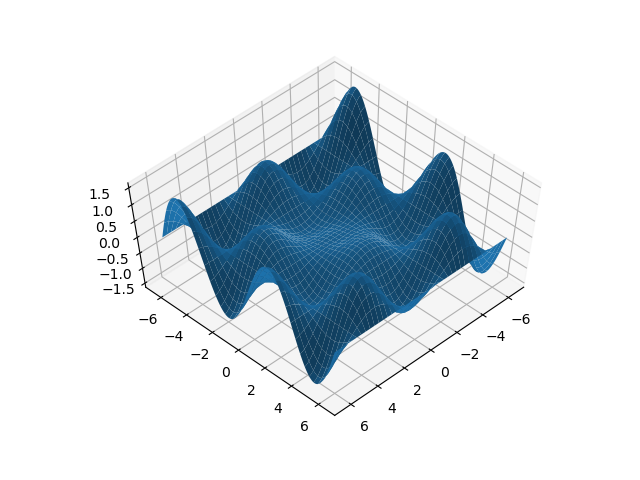
\includegraphics[width=.6\linewidth]{./gfx/np-wave}
	\captionof{figure}{Wellen auf Wasser}
\end{center}
\end{tcolorbox}

\subsection{Vergleiche}
Auch Relationen (\texttt{==}, \texttt{<}, etc.) sind auf NumPy-Arrays definiert; auch hier wird Elementweise gearbeitet. Ergebnis ist also ein Array von \inPy{bool}s, das markiert, welche Array-Elemente die angegebene Relation erfüllen. Es sei daran erinnert, dass Arrays von \inPy{bool}s wiederum zum \enquote{Filtern} von NumPy-Arrays genutzt werden können\footnote{Das Unter-Modul \texttt{numpy.random} wird in Abschnitt \ref{sec:NumPy-Random} besprochen. Im folgenden Beispiel wird die Funktion \texttt{randint(low, high, size)} verwendet, die ein NumPy-Array der Länge \texttt{size} mit \inPy{int}-Werten zwischen einschließlich \texttt{low} und ausschließlich \texttt{high} erzeugt. Ich denke, Sie können mit diesem Wissen bereits sehr gut verstehen, wie der Code funktioniert.}.

\begin{codebox}[Beispiel: Relationen auf NumPy-Arrays]
\begin{minted}[linenos]{python3}
import numpy as np

data = np.random.randint(-5, 5, 20))
positive = data > 0

print("all data        :", data)
print("mask            :", positive)
print("pos. data points:", data[positive])
\end{minted}
\end{codebox}

\begin{cmdbox}[Ausgabe: Relationen auf NumPy-Arrays]
\begin{minted}{text}
all data        : [-2 -2 -2  2  5  1  2  4  2 -1 -5  0  4  2  3  3  3  5  2 -1]
mask            : [False False False  True  True  True  True  True  True False 
  False False  True  True  True  True  True  True  True False]
pos. data points: [2 5 1 2 4 2 4 2 3 3 3 5 2]
\end{minted}
\end{cmdbox}

Um zu testen, ob zwei NumPy-Arrays als Ganzes gleich sind, kann \texttt{array\_equal} genutzt werden. Es wird direkt die Gleichheit geprüft, \ie \texttt{np.array\_equal(A, B)} gibt genau dann \inPy{True} zurück, wenn \texttt{A-shape == B.shape} \emph{und} wenn alle Einträge in \texttt{A} mit denen in \texttt{B} übereinstimmen. Andernfalls ist der Rückgabewert \inPy{False}.

Für andere Vergleiche als die Gleichheit können \texttt{all} und \texttt{any} benutzt werden. Beide erwarten ein NumPy-Array von \inPy{bool}s, über die gesammelt das logische \inPy{and} bzw. \inPy{or} ausgeführt wird. Als Mensch gesprochen: die Funktionen geben \inPy{True} zurück, wenn \emph{alle} bzw. \emph{mindestens ein Element} des Arrays schon \inPy{True} war. Mit dem optionalen Parameter \texttt{axis} können \texttt{all} und \texttt{any} dazu angewiesen werden, nur entlang einer Achse zu operieren.

\begin{codebox}[Beispiel: \texttt{array\_equal}{,} \texttt{all} und \texttt{any}]
\begin{minted}[linenos]{python3}
data = np.random.randint(-5, 5, (3, 3))
copy = data.copy()

print(data)
print()

print("Original and copy are identical:", np.array_equal(data, copy))
print("Alternative form of same test  :", np.all(data == copy))
   # hierbei wird shape NICHT verglichen!
print()

for i, truth in enumerate( np.any(data < 0, axis=0) ) :
    print(f"column {i} has{'' if truth else ' no'} negatie entries.")
print()

for i, truth in enumerate( np.any(data < 0, axis=1) ) :
    print(f"row {i} has{'' if truth else ' no'} negatie entries.")
\end{minted}
\end{codebox}

\begin{cmdbox}[Ausgabe: \texttt{array\_equal}{,} \texttt{all} und \texttt{any}]
\begin{minted}{text}
[[-3 -5 -1]
 [ 3  0  1]
 [ 0 -2  4]]

Original and copy are identical: True
Alternative form of same test  : True

column 0 has negatie entries.
column 1 has negatie entries.
column 2 has negatie entries.

row 0 has negatie entries.
row 1 has no negatie entries.
row 2 has negatie entries.
\end{minted}
\end{cmdbox}

\section{Reduktion}
NumPy bietet viele Lösungen für Operationen auf Arrays. Wir kennen bereits Möglichkeiten, eine Berechnung für jedes Element eines Arrays auszuführen und dabei ein neues Array von Werten zu erhalten. Oft wollen wir aber die Werte nicht isoliert betrachten, sondern aus ihrer Gesamtheit einen einzigen Wert wie \eg. den Durchschnitt generieren. Auch für solche \emph{Reduktionen} bietet NumPy vorgefertigte Lösungen.

Natürlich kennen wir bereits Möglichkeiten, solche Reduktionen mit Python-Mitteln durchzuführen. Pythons \inPy{sum} und \inPy{len} geben Summe und Länge eines Arrays aus, und können auch auf NumPy-Arrays angewandt werden. Da diese Funktionen jedoch für sehr viele verschiedenartige Strukturen funktionieren sollen, konnten sie nicht weit optimiert werden. Aus diesem Grund bringt NumPy seine eigenen Funktionen mit, die die spezielle Struktur von NumPy-Arrays ausnutzen, und so eine Aufgabe sehr schnell lösen.

\begin{hintbox}[Exkursion: Zeitmessung mit \texttt{time}]
Das Modul \texttt{time} erlaubt -- wie es der Name schon suggeriert --, in Python mit Zeiten umzugehen. Neben Funktionen zur Formatierung von Zeitpunkten als Strings und Berechnung von Zeit-Abständen existiert die Funktion \texttt{time}, die das aktuelle Datum und Uhrzeit als Rückgabewert liefert. Diese Information wird in einer einzigen Fließkommazahl codiert, welche als Anzahl der Sekunden seit Mitternacht, erster Januar 1970 zu deuten ist. Vorteil dieser Konvention ist, dass solche \emph{Zeitstempel} einfach voneinander subtrahiert werden können, um \emph{Zeitabstände} zu erfahren.

Um den Zeitbedarf eines Algorithmus experimentell zu ermitteln hält man sich häufig an das folgende Schema:
\begin{codebox}[Schema: Zeitbedarf ermitteln]
\begin{minted}{python3}
import time

R = 1000

tic = time.time()
for run in range(R) :
    # Algorithmus
toc = time.time()

print(f"it took {toc - tic} second to run the algorithm {R} times")
\end{minted}
\end{codebox}

Die sehr kleinen Zeiten, die ein Computeralgorithmus zur Durchführung braucht, sind oft starken Schwankungen unterworfen. Um diese Schwankungen auszugleichen, wird meist nicht der Zeitbedarf für \emph{einen} Durchlauf ermittelt, sondern der \emph{durchschnittliche} Zeitbedarf für \emph{sehr viele} Durchläufe des Algorithmus. Daraus erklärt sich die Schleife über \texttt{run} im oben gezeigten Schema.
\end{hintbox}

Ein kurzes Script illustriert, wie viel größer der Zeitaufwand ohne NumPy-Funktionen ist:

\begin{codebox}[Beispiel: Zeitbedarf Array-Summation mit NumPy und Python]
\begin{minted}[linenos]{python3}
import numpy as np
import time

N = 10000
R =  2000
X = np.linspace(0, 100, N)

print(f"taking the time for summation of {N} values, Python-Style...",
      end="", flush=True)
tic = time.time()
for run in range(R) :
  s = sum(X)
toc = time.time()
print("done")
tPython = toc - tic

print(f"taking the time for summation of {N} values, NumPy-Style...",
      end="", flush=True)
tic = time.time()
for run in range(R) :
  s = np.sum(X)
toc = time.time()
print("done")
tNumpy = toc - tic

print()
print(f"Measured {tPython*1000/R:5.3f} milliseconds using the Python-Method")
print(f"Measured {tNumpy *1000/R:5.3f} milliseconds using the NumPy-Method")
print(f"NumPy is {tPython/tNumpy:5.1f} times faster than native Python")
\end{minted}
\end{codebox}
%
\begin{cmdbox}[Ausgabe: Zeitbedarf Array-Summation mit NumPy und Python]
\begin{minted}{text}
taking the time for summation of 10000 values, Python-Style...done
taking the time for summation of 10000 values, NumPy-Style...done

Measured 1.589 milliseconds using the Python-Method
Measured 0.008 milliseconds using the NumPy-Method
NumPy is 211.5 times faster than native Python
\end{minted}
\end{cmdbox}

Bei mehrdimensionalen Arrays wird standardmäßig über alle Einträge summiert. Optional kann aber auch der \inPy{int}-Parameter \texttt{axis} mitgegeben werden. Dieser gibt an, über die wievielte Dimension summiert werden soll. Auch der Rückgabetyp des hierbei entstehenden NumPy-Arrays kann über das optionale Argument \texttt{dytpe} bestimmt werden.

\begin{tcbraster}[raster columns=2,
                  raster equal height,
                  nobeforeafter,
                  raster column skip=0.5cm]
\begin{codebox}[Beispiel: Summation in mehr Dimensionen]
\begin{minted}[linenos]{python3}
import numpy as np

npTab = np.array([[1, 2], [3, 4]])

print( np.sum(npTab) )
print( np.sum(npTab, axis=0) )
print( np.sum(npTab, axis=1) )
\end{minted}
\end{codebox}
%
\begin{cmdbox}[Ausgabe: Summation in mehr Dimensionen]
\begin{minted}{text}
10
[4 6]
[3 7]
\end{minted}
\end{cmdbox}
\end{tcbraster}

Das eben zu \texttt{np.sum} gesagte gilt so gleichermaßen auch für \texttt{np.prod} (Produkt der Werte eines NumPy-Arrays).

Der Mittelwert eines NumPy-Arrays kann über \texttt{mean} ermittelt werden. Auch hier können optional \texttt{axis} und \texttt{dtype} mit angegeben werden. Eine Erweiterung von \texttt{mean} stellt \texttt{average} dar. Diesem kann ein optionaler Parameter \texttt{weights} mitgegeben werden. Wie der Name nahelegt, handelt es sich hierbei um Gewichte für die einzelnen Werte des Daten-Arrays. Der Aufruf \texttt{np.average(a, weights=w)} berechnet also
\[ \frac{\sum_i a_i w_i}{\sum_i w_i}\]

Der Nenner in diesem Ausdruck -- die sogenannte \emph{Zustandssumme} oder \emph{Partition Function} -- kann mit demselben Befehl in Erfahrung gebracht werden. Wird das optionale Argument \inPy{returned=True} mit übergeben, so ist der Rückgabewert ein \inPy{tuple} aus gewichtetem Durchschnitt und Zustandssumme\footnote{Ich \emph{hasse} Thermodynamik.}:

\begin{codebox}[Beispiel: Durchschnittgeschwindigkeit in Wasserstoff (Statistische Physik)]
\begin{minted}[linenos]{python3}
kB = 1.380649e-23         # Boltzmann constant
T  = 300                  # Temperature in Kelvin
m  = 2 * 1.6735575e-27    # hydrogen molecule mass in kg

velocities = np.linspace(0, 5000, 50000)
energies   = m/2 * velocities**2
w = np.exp(-energies / (kB * T))

vMean, Z = np.average(velocities, weights=w, returned=True)

print("weighted average:", vMean, "m/s")
print("partition function:", Z)
\end{minted}
\end{codebox}
%
\begin{cmdbox}[Ausgabe: Durchschnittgeschwindigkeit in Wasserstoff (Statistische Physik)]
\begin{minted}{text}
weighted average: 887.5169329420108 m/s
partition function: 13942.18222351434
\end{minted}
\end{cmdbox}

Eng mit dem Mittelwert verknüpft sind der \emph{Median} und die \emph{Standardabweichung}. 

\begin{hintbox}[Median und Standardabweichung]
Der Median wird oft auch \emph{Mitte\textbf{n}wert} (im Gegensatz zum \emph{Mitte\textbf{l}wert}) genannt. Wenn man die Werte einer Stichprobe aufsteigend ordnet, so handelt es sich um den Wert \enquote{in der Mitte der geordneten Liste}. Bei einer Liste mit gerader Anzahl von Werten ist es das arithmetische Mittel (der Mittelwert) aus den beiden Werten in der Mitte der Liste.

Beispiel 1:\\
Seien die folgenden Werte gegeben: \tab $1, 5, 8, 5, 2, 1, 4, 3, 1$\\
Sortiert man diese Liste, so erhält man: \tab $1, 1, 1, 2, 3, 4, 5, 5, 8$\\
der Median dieser Liste aus 9 Zahlen ist also der fünfte Wert der sortierten Liste, also die 3.

Beispiel 2:\\
Seien die folgenden Werte gegeben: \tab $1, 5, 8, 5, 2, 4, 3, 1$\\
Sortiert man diese Liste, so erhält man: \tab $1, 1, 2, 3, 4, 5, 5, 8$\\
der Median dieser Liste aus 8 Zahlen ist also der Mittelwert aus dem vierten und fünften Wert der sortierten Liste, also $\frac{3+4}{2} = 3.5$.

Die \emph{Standardabweichung} kann als Streuung um den Mittelwert verstanden werden. Es stellt sich heraus, dass die meisten elementaren Prozesse in der echten Welt einer \emph{Normalverteilung} folgen. Gegeben eine Menge von $N$ Werten $x_i$ mit Mittelwert $\mu$, finden wir diese Streuung $\sigma$ nach der Formel:
\[ \sigma = \sqrt{\frac{\sum_{i=1}^N (x_i - \mu)^2 }{N}} \]
Die Aussage dieses Wertes $\sigma$ ist anschaulich, dass die überwiegende Mehrhet der Werte\footnote{etwa 68\%} innerhalb von $\mu \pm \sigma$ liegen.
\end{hintbox}

Median und Standardabweichung können mit den Befehlen \texttt{median} und \texttt{std} berechnet werden. Wie schon zuvor erlaubt der optionale Parameter \texttt{axis} es, beispielsweise Zeilen- oder Spaltenweise zu arbeiten; über \texttt{dtype} kann der Datentyp des Ausgabe-Arrays bestimmt werden.

Der Vollständigkeit halber sei auch auf die NumPy-Versionen von \texttt{min} und \texttt{max} hingewiesen werden, die derselben Logik folgen und Minimun und Maximum eines (Sub-)Arrays ermitteln. Wo nicht das Minimum/Maximum selbst relevant ist, sondern seine Position im Array, können die Befehle \texttt{argmin} und \texttt{argmax} eingesetzt werden:

\begin{codebox}[Beispiel: Minimum und Maximum]
\begin{minted}[linenos]{python3}
npTab = np.array([[1, 2], [3, 4]])

print( "min:", np.min(npTab), "at index", np.argmin(npTab) )
print( "max:", np.max(npTab), "at index", np.argmax(npTab) )
print( "min (axis=0):", np.min(npTab, axis=0), "at", np.argmin(npTab, axis=0) )
print( "max (axis=0):", np.max(npTab, axis=0), "at", np.argmax(npTab, axis=0) )
\end{minted}
\end{codebox}
%
\begin{cmdbox}[Ausgabe: Minimum und Maximum]
\begin{minted}{text}
min: 1 at index 0
max: 4 at index 3
min (axis=0): [1 2] at [0 0]
max (axis=0): [3 4] at [1 1]
\end{minted}
\end{cmdbox}

\section{Umformungen an NumPy-Arrays}
Oft erhalten wir die Daten, mit denen wir arbeiten wollen, nicht im für die weiteren Schritte günstigsten Form. Es kann sein, dass unsere Quelldaten umsortiert, besonders angeordnet, ergänzt oder verschoben werden müssen, bevor wir sinnvoll damit arbeiten können. Die in diesem Abschnitt vorgestellten Befehle helfen uns dabei. Sie stellen eine Unterauswahl der Befehle dar, die auf \url{https://numpy.org/doc/stable/reference/routines.array-manipulation.html} aufgelisteten sind.

\subsection{Arrays Verbinden und Trennen}
Auf Python-\inPy{list}s ist die Addition als Hintereinanderhängen der Listen definiert. Bei NumPy-Arrays dagegen handelt es sich um die Elementweise Addition der Werte. Um die Verkettung von NumPy-Arrays zu erreichen können wir verschiedene Befehle benutzen; das Allzweck-Tool zum Verketten ist der Befehl \texttt{concatenate}. Übergeben wird ein \inPy{tuple}\footnote{beachten Sie daher das zusätzliche Paar von Klammern ()!} von NumPy-Arrays, die zu einem einzigen Array zusammengesetzt werden sollen. Optional kann der Parameter \texttt{axis} übergeben werden, der bestimmt, \enquote{in welcher Richtung} ein zusätzliches Array angehängt wird. Der Wert von \texttt{axis} kann auch \inPy{None} sein; in diesem Fall wird aus den Arrays eine eindimensionale Liste erstellt. Alle zu verkettenden Arrays müssen in der gewählten Dimension dieselbe Anzahl von Einträgen haben. Der Default-Wert für \texttt{axis} ist \inPy{0}.

\begin{codebox}[Beispiel: \texttt{concatenate}]
\begin{minted}[linenos]{python3}
import numpy as np

a = np.array([[1, 2], [3, 4]])
b = np.array([[5, 6]])
c = np.array( [7, 8] )

print( np.concatenate((a, b))             , end="\n\n" )
print( np.concatenate((a, b)  , axis=0)   , end="\n\n" )
print( np.concatenate((a, b.T), axis=1)   , end="\n\n" )
print( np.concatenate((a, b)  , axis=None), end="\n\n" )
\end{minted}
\end{codebox}

\begin{cmdbox}[Ausgabe: \texttt{concatenate}]
\begin{minted}{text}
[[1 2]
 [3 4]
 [5 6]]
 
[[1 2]
 [3 4]
 [5 6]]

[[1 2 5]
 [3 4 6]]

[1 2 3 4 5 6]
\end{minted}
\end{cmdbox}

Um beim Verketten eine neue Dimension einzuführen können wir den Befehl \texttt{stack} benutzen. Prinzipiell gilt dasselbe, das schon zu \texttt{concatenate} gesagt wurde. Während \texttt{concatenate} aus zwei $N$-dimensionalen Objekten wieder ein $N$-dimensionales Objekt erzeugt, ist das Erbebnis von \texttt{stack} $N+1$-dimensional. Entsprechend darf der Wert von \texttt{axis} hier auch zwischen $0$ und $N$ liegen.

\begin{codebox}[Beispiel: \texttt{stack}]
\begin{minted}[linenos, firstnumber=10]{python3}
# ...

print( np.stack((c, c))        , end="\n\n" )
print( np.stack((c, c), axis=0), end="\n\n" )
print( np.stack((c, c), axis=1), end="\n\n" )
print( np.stack((a, a))        , end="\n\n" )
\end{minted}
\end{codebox}

\begin{cmdbox}[Ausgabe: \texttt{stack}]
\begin{minted}{text}
[[ 0 -1]
 [ 0 -1]]

[[ 0 -1]
 [ 0 -1]]

[[ 0  0]
 [-1 -1]]

[[[1 2]
  [3 4]]

 [[1 2]
  [3 4]]]
\end{minted}
\end{cmdbox}

Ebenso, wie NumPy-Arrays zusammengefügt werden können, ist es möglich, diese auch zu zerteilen. Hierzu dient der Befehl \texttt{split}. Übergeben werden muss zum einen das zu zerteilende Array, sowie eine Information, wie es zerschnitten werden soll. Dies kann entweder in Form eines \inPy{int}s oder eines eindimensionalen \inPy{int}-Containers (\inPy{list}, \inPy{tuple}, NumPy-Array, ...) geschehen.

Wird ein \inPy{int} übergeben, so legt dieser die Anzahl der entstehenden Blöcke fest. NumPy versucht, das Array in Blöcke gleicher Größe zu zerschneiden. Ist es nicht möglich, eine Array restlos zu zerteilen (\eg: ein Array mit 5 Elementen soll in 3 Teile zerschnitten werden), wird eine Fehlermeldung ausgelöst.

Bei einer Liste dagegen versteht NumPy die Listen-Einträge als Punkte, an denen geschnitten werden soll. \inPy{[2, 4]} teilt ein Array \texttt{A} beispielsweise in drei Blöcke: \texttt{A[:2]}, \texttt{A[2:4]} und \texttt{A[4:]}.

Wie üblich kann auch wieder über \texttt{axis} festgelegt werden, in welcher Richtung geschnitten werden soll.

\begin{codebox}[Beispiel: \texttt{split}]
\begin{minted}[linenos]{python3}
data = np.array([[1, 2, 3, 4, 5], [6, 7, 8, 9, 0]])

print( np.split(data, 2) )
print( np.split(data, (2, 4), axis=1) )
\end{minted}
\end{codebox}

\begin{cmdbox}[Ausgabe: \texttt{split}]
\begin{minted}{text}
[array([[1, 2, 3, 4, 5]]), array([[6, 7, 8, 9, 0]])]
[array([[1, 2],
       [6, 7]]), array([[3, 4],
       [8, 9]]), array([[5],
       [0]])]
\end{minted}
\end{cmdbox}

\begin{tcbraster}[raster columns=2,
                  raster equal height,
                  nobeforeafter,
                  raster column skip=0.15cm]
\begin{tcolorbox}[title=\texttt{np.split(data, 2)}]
\begin{align*}
	\begin{pmatrix}
		1 & 2 & 3 & 4 & 5\\
		6 & 7 & 8 & 9 & 0
	\end{pmatrix}
&\thus&&
	\begin{matrix}
	\begin{pmatrix}
		1 & 2 & 3 & 4 & 5
	\end{pmatrix},
	\\
	\begin{pmatrix}
		6 & 7 & 8 & 9 & 0
	\end{pmatrix}
	\end{matrix}
\end{align*}
\end{tcolorbox}
%
\begin{tcolorbox}[title=\texttt{np.split(data, (2, 4), axis=1)}]
\begin{align*}
	\begin{pmatrix}
		1 & 2 & 3 & 4 & 5\\
		6 & 7 & 8 & 9 & 0
	\end{pmatrix}
&\thus&&
	\begin{matrix}
	\begin{pmatrix}
		1 & 2 \\ 6 & 7
	\end{pmatrix},
	\begin{pmatrix}
		3 & 4 \\ 8 & 9
	\end{pmatrix},
	\begin{pmatrix}
		5 \\ 0
	\end{pmatrix}
	\end{matrix}
\end{align*}
\end{tcolorbox}
\end{tcbraster}

\subsection{Elemente Einfügen und Löschen}
Mit dem Befehl \texttt{insert} können in NumPy-Arrays zusätzliche Spalten eingefügt werden. Es folgt der Syntax
\begin{center}
	\inPy{np.insert(array, where, what, axis=0)}
\end{center}

Dabei ist...
\begin{itemize}
\item \texttt{array} das NumPy-Array, in das eine Spalte eingefügt werden soll
\item \texttt{where} der Index oder die Indices der Spalten, die eingefügt werden sollen. Es kann sich hierbei also um einen \inPy{int} oder einen Container von
	\inPy{int}s handeln.
\item \texttt{what} das Element oder die Elemente, die eingefügt werden sollen. Es kann sich hierbei um einen einzelnen Wert handeln, der dann in jedes Feld der
	eingefügten Spalten geschrieben wird, oder ein Container, der alle zu schreibenden Werte enthält.
\item \texttt{axis} in seiner gewohnten Bedeutung zu verstehen.
\end{itemize}

\begin{codebox}[Beispiel: \texttt{insert}]
\begin{minted}[linenos]{python3}
data = np.array([0, 1, 2, 3], [4, 5, 6, 7])
idx = (1, 3)
print( np.insert(data, idx, 999, axis=1) )
print()

data = np.array([[1, 1], [2, 2], [3, 3]])
print( np.insert(data, 1, 5) )
print()

print( np.insert(data, 1, 5, axis=1) )
print( np.insert(data, [1], [[1],[2],[3]], axis=1) )
\end{minted}
\end{codebox}

\begin{cmdbox}[Ausgabe: \texttt{insert}]
\begin{minted}{text}
[[  0 999   1   2 999   3]
 [  4 999   5   6 999   7]]
 
[1 5 1 2 2 3 3]

[[1 5 1]
 [2 5 2]
 [3 5 3]]
 
[[1 1 1]
 [2 2 2]
 [3 3 3]]
\end{minted}
\end{cmdbox}

Ebenso können Spalten aus NumPy-Arrays mit \texttt{delete} gelöscht werden. Analog zu \texttt{insert} lautet dabei die Syntax:
\begin{center}
	\inPy{np.delete(array, where, axis=0)}
\end{center}
\ie dieselbe Logik wie für \texttt{insert} lässt sich auch auf \texttt{delete} anwenden.

\subsection{Größe und Form Ändern}
Die \emph{Methode} \texttt{resize} erlaubt es, die Größe eines Arrays nach der Erstellung zu ändern. Übergeben wird ein \inPy{tuple}, der die neue Größe des Arrays angibt. Vergrößert sich das Array beim Aufruf von \texttt{resize}, so werden Nullen eingefügt; bei Verkleinerungen werden einfach Werte \enquote{abgeschnitten}. In beiden Fällen behält NumPy die \emph{vektorisierte Datenmenge} des Arrays bei:

Die Matrix:
\[ A = \begin{pmatrix}
		1 & 2 \\ 3 & 4
\end{pmatrix} \]
liegt vektorisiert vor als
\[ \begin{matrix}
	1 & 2 & 3 & 4
\end{matrix} \]
Nach einem Aufruf von \texttt{A.resize((2, 3))}\footnote{beachten Sie, dass \emph{zwei} Klammern nötig sind, da die \texttt{shape} als \inPy{tuple} übergeben werden muss!} werden zwei Nullen angefügt, um insgesamt 6 Zahlen im Datenpuffer zu erzeugen; wir finden also
\[ \begin{matrix}
	 1 & 2 & 3 & 4 & 0 & 0
\end{matrix} \]
die gelesen werden als
\[ \begin{pmatrix}
	1 & 2 & 3 \\ 4 & 0 & 0
\end{pmatrix} \]

Ebenso erhalten wir (ausgehen von der 2x2-Matrix) nach Aufruf von \texttt{A.reshape((2, 1))} die Matrix:
\[ \begin{pmatrix}
	1 \\ 2
\end{pmatrix} \]

Die Methode \texttt{reshape} funktioniert genauso wie \texttt{resize}, ändert aber nicht die Gesamt-Datenmenge. Stattdessen wird eine Fehlermeldung erzeugt, wenn die neue Form mehr oder weniger Daten als das ursprüngliche Array enthält. Anders als \texttt{resize} wird die neue Größe aber nicht direkt auf das Array angewandt, sondern gilt nur für eine \emph{Kopie}. Ist \texttt{A} eine $2 \times 3$-Matrix, so ist nach dem Aufruf von \texttt{A.reshape((3, 2))} immer noch von der Form $2 \times 3$. Um die Änderung auf \texttt{A} anzuwenden, muss entweder \texttt{A = A.reshape((3, 2))} oder \texttt{np.reshape(A, (3, 2))} benutzt werden.

\begin{codebox}[Beispiel: \texttt{reshape}]
\begin{minted}[linenos]{python3}
data = np.arange(8).reshape((2,4))
print(data)

data.reshape((4, 2))     # ohne Effekt!
print( data )

data.reshape((3, 3))     # löst Fehlermeldung aus
\end{minted}
\end{codebox}
%
\begin{cmdbox}[Ausgabe: \texttt{reshape}]
\begin{minted}{text}
[[0 1 2 3]
 [4 5 6 7]]
[[0 1 2 3]
 [4 5 6 7]]
Traceback (most recent call last):
  File "<stdin>", line 9, in <module>
ValueError: cannot reshape array of size 8 into shape (3,3)
\end{minted}
\end{cmdbox}

Die Methode \texttt{flatten} liefert immer ein eindimensionales NumPy-Array, das der vektorisierten Form entspricht, in die Matrix bzw. der Tensor im Speicher vorliegt. Optional kann der Parameter \texttt{order} übergeben werden, und so mit \inPy{'C'} eine Vektorisierung in Row-Major-Form oder mit \inPy{'F'} eine solche in Column-Major-Form erzeugt werden:

\begin{tcbraster}[raster columns=2,
                  raster equal height,
                  nobeforeafter,
                  raster column skip=0.5cm]
\begin{codebox}[Beispiel: \texttt{flatten}]
\begin{minted}[linenos]{python3}
data = np.arange(8).reshape((2,4))
data.flatten()  # ohne Effekt

print(data)
print(data.flatten())
print(data.flatten('F'))
\end{minted}
\end{codebox}
%
\begin{cmdbox}[Ausgabe: \texttt{flatten}]
\begin{minted}{text}
[[0 1 2 3]
 [4 5 6 7]]
[0 1 2 3 4 5 6 7]
[0 4 1 5 2 6 3 7]
\end{minted}
\end{cmdbox}
\end{tcbraster}

\subsection{Pattern aus Arrays}
Manchmal finden wir uns in der Situation, dass Teile einer Matrix oder eines Tensors sich wiederholen. In diesem Fall können wir aus den Sub-Pattern den gesamten Tensor mit dem Befehl \texttt{repeat} erstellen. Er folgt der Syntax
\begin{center}
	\inPy{np.repeat(what, repeats, axis=None)}
\end{center}
wobei \texttt{what} das zu wiederholende Subpattern ist. \texttt{repeats} kann ein \inPy{int} oder ein \inPy{tuple} von \inPy{int}s, der angibt, wie oft die Elemente von \texttt{what} wiederholt werden sollen. \texttt{axis} steuert hier wieder, in welcher Richtung die Wiederholungen stattfinden.

\begin{tcbraster}[raster columns=2,
                  raster equal height,
                  nobeforeafter,
                  raster column skip=0.5cm]
\begin{codebox}[Beispiel: \texttt{repeat}]
\begin{minted}[linenos]{python3}
print(np.repeat(3, 4))

x = np.array([[1,2],[3,4]])

print(np.repeat(x, 2))
print(np.repeat(x, 3, axis=1))
print(np.repeat(x, [1, 2], axis=0))
\end{minted}
\end{codebox}
%
\begin{cmdbox}[Ausgabe: \texttt{repeat}]
\begin{minted}{text}
[3 3 3 3]
[1 1 2 2 3 3 4 4]
[[1 1 1 2 2 2]
 [3 3 3 4 4 4]]
[[1 2]
 [3 4]
 [3 4]]
\end{minted}
\end{cmdbox}
\end{tcbraster}

Ähnlich wie \texttt{repeat} funktioniert auch \texttt{tile}: Auch hier wird ein Sub-Pattern wiederholt, kann aber auch in mehrere Richtungen zugleich ausgedehnt werden. Die Syntax lautet:

\begin{center}
	\inPy{np.tile(what, repeats)}
\end{center}
Auch hier wieder ist \texttt{what} das zu wiederholende Sub-Pattern. \texttt{repeats} ist wieder ein \inPy{int} oder \inPy{tuple}, der jetzt aber die Wiederholungen \emph{je Richtung} angibt:

\begin{tcbraster}[raster columns=2,
                  raster equal height,
                  nobeforeafter,
                  raster column skip=0.5cm]
\begin{codebox}[Beispiel: \texttt{tile}]
\begin{minted}[linenos, firstnumber=9]{python3}
# ...

print( np.tile(x, 2) )
print( np.tile(x, (2, 1)) )
\end{minted}
\end{codebox}
%
\begin{cmdbox}[Ausgabe: \texttt{tile}]
\begin{minted}{text}
[[1 2 1 2]
 [3 4 3 4]]
[[1 2]
 [3 4]
 [1 2]
 [3 4]]
\end{minted}
\end{cmdbox}
\end{tcbraster}

Manche interessante Matrizen bestehen aus Komponenten, die sich durch Verschiebung eines einfacheren Elements ergeben. Betrachten Sie die folgende Matrix\footnote{Es handelt sich hier um eine Darstellung der \emph{Ableitung mit zyklischen Randbedingungen} in der \emph{Finite Elemente Methode}.}:
\[
\frac{1}{2}
\begin{pmatrix}
	 0 &  1 &  0 &  0 &  0 & -1 \\
	-1 &  0 &  1 &  0 &  0 &  0 \\
   0 & -1 &  0 &  1 &  0 &  0 \\
   0 &  0 & -1 &  0 &  1 &  0 \\
   0 &  0 &  0 & -1 &  0 &  1 \\
   1 &  0 &  0 &  0 & -1 &  0 \\
\end{pmatrix} 
=
\frac{1}{2}
\begin{pmatrix}
	 0 &  1 &  0 &  0 &  0 &  0 \\
	 0 &  0 &  1 &  0 &  0 &  0 \\
   0 &  0 &  0 &  1 &  0 &  0 \\
   0 &  0 &  0 &  0 &  1 &  0 \\
   0 &  0 &  0 &  0 &  0 &  1 \\
   1 &  0 &  0 &  0 &  0 &  0 \\
\end{pmatrix}
+
\frac{1}{2}
\begin{pmatrix}
	 0 &  0 &  0 &  0 &  0 & -1 \\
	-1 &  0 &  0 &  0 &  0 &  0 \\
   0 & -1 &  0 &  0 &  0 &  0 \\
   0 &  0 & -1 &  0 &  0 &  0 \\
   0 &  0 &  0 & -1 &  0 &  0 \\
   0 &  0 &  0 &  0 & -1 &  0 \\
\end{pmatrix}
\]

Die Zerlegung in eine Summe erinnert an Diagonalmatrizen, weicht von diesen jedoch durch die beiden Einträge in der rechten oberen bzw. linken unteren Ecke von diesen ab. Wir erhalten die Zerlegung, indem wir eine Diagonalmatrix um eine Spalte nach links bzw. rechts verschieben; \enquote{überstehende} Spalten werden dabei am anderen Ende wieder angehängt:

\[\begin{pmatrix}
   1 &  0 &  0 &  0 &  0  &  \color{blue}0 \\
   0 &  1 &  0 &  0 &  0  &  \color{blue}0 \\
   0 &  0 &  1 &  0 &  0  &  \color{blue}0 \\
   0 &  0 &  0 &  1 &  0  &  \color{blue}0 \\
   0 &  0 &  0 &  0 &  1  &  \color{blue}0 \\
   0 &  0 &  0 &  0 &  0  &  \color{blue}1 \\
\end{pmatrix}
\thus
\begin{pmatrix}
   \color{blue} 0 &  1 &  0 &  0 &  0 &  0 \\
   \color{blue} 0 &  0 &  1 &  0 &  0 &  0 \\
   \color{blue} 0 &  0 &  0 &  1 &  0 &  0 \\
   \color{blue} 0 &  0 &  0 &  0 &  1 &  0 \\
   \color{blue} 0 &  0 &  0 &  0 &  0 &  1 \\
   \color{blue} 1 &  0 &  0 &  0 &  0 &  0 \\
\end{pmatrix}
\]

Genau diese Funktion erfüllt der Befehl \texttt{roll}. Erwartet wird, um wie viele Schritte die gegebene Matrix verschoben werden soll; optional kann außerdem über den Parameter \texttt{axis} angegeben werden, in Richtung welcher Achse die Matrix verschoben werden soll. Die obige Matrix lässt sich damit in Python so sehr schnell erstellen:

\begin{codebox}[Beispiel: \texttt{roll}]
\begin{minted}[linenos]{python3}
import numpy as np

D = 5
derivative = 0.5 * ( np.roll(np.diag(np.ones(D)),  1, axis=1) - \
                     np.roll(np.diag(np.ones(D)), -1, axis=1) )
print(derivative)
\end{minted}
\end{codebox}
%
\begin{cmdbox}[Ausgabe: \texttt{roll}]
\begin{minted}{text}
[[ 0.   0.5  0.   0.  -0.5]
 [-0.5  0.   0.5  0.   0. ]
 [ 0.  -0.5  0.   0.5  0. ]
 [ 0.   0.  -0.5  0.   0.5]
 [ 0.5  0.   0.  -0.5  0. ]]
\end{minted}
\end{cmdbox}

\subsection{Sortieren und Suchen}
Wie Sie sich vorstellen können, hat NumPy auch seine eigene, optimierte Sortierfunktion. Diese kann sowohl über den \emph{Befehl} \texttt{sort} als auch über die \emph{Methode} \texttt{sort} aufgerufen werden. Unterschied der beiden ist, dass der Befehl \texttt{sort} eine sortierte Kopie des NumPy-Arrays erstellt, während die Methode \emph{in place} arbeitet, also das Array selbst verändert. Der Befehl arbeitet also wie \inPy{sorted}, während die Methode so arbeitet wie \inPy{list.sort}.

Für Mehrdimensionale Objekte kann wieder der optionale Parameter \texttt{axis} mitgegeben werden, der angibt, ob Zeilen-, Spalten-, Schichten-, ...-weise sortiert wird. Per Default wird entlang der letzten Achse sortiert. Ist \inPy{axis=None}, so ordnet NumPy die vektorisierten Daten des Arrays um, ungeachtet der zugrundeliegenden Struktur.

Ein Sortierschlüssel kann in NumPy leider nicht mitgegeben werden\footnote{Genauer: NumPy erlaubt zwar, Arrays von Listen nach ausgewählten Feldern zu sortieren. Das Anwenden einer Funktion auf die Array-Elemente dagegen ist nicht möglich. Auf diese Möglichkeit soll hier der Übersichtlichkeit halber aber nicht eingegangen werden. Lesen Sie sich hierzu den Eintrag von \texttt{help(np.sort)} durch, oder sehen Sie sich die Online-Doku unter \url{https://numpy.org/doc/stable/reference/generated/numpy.sort.html} an, falls Sie mehr erfahren wollen.}. Für die üblichen Anwendungsflälle ist dies aber auch nicht nötig -- NumPy hat seine Stärken im Umgang mit Zahlen, die nur selten in einer anderen als der \enquote{natürlichen} Reihenfolge sortiert werden müssen.

\begin{codebox}[Beispiel: \texttt{sort}]
\begin{minted}[linenos]{python3}
data = np.array([[1,4], [3,1]])

print( np.sort(data) )   # Sortiere nach letzter Dimension (Spaltenweise)
print(         data  )   # Sortieren hatte keinen Einfluss auf data selbst
print( data.sort()   )   # Sortieren nach letzter Dimension, in place
print(         data  )   # Effekt jetzt sichtbar
print()

print( np.sort(data, axis=None) )    # geplättetes Array sortieren
print( np.sort(data, axis=0)    )    # Zwelenweise sortieren
print(derivative)
\end{minted}
\end{codebox}
%
\begin{cmdbox}[Ausgabe: \texttt{sort}]
\begin{minted}{text}
[[1 4]
 [1 3]]
[[1 4]
 [3 1]]
None
[[1 4]
 [1 3]]

[1 1 3 4]
[[1 3]
 [1 4]]
\end{minted}
\end{cmdbox}

Wo es tatsächlich nötig ist, ein NumPy-Array nach einem Kriterium $f$ zu sortieren, wie das mit Pythons \texttt{sorted(array, key=f)} möglich wäre, kann auch der Befehl \texttt{argsort} verwendet werden. Dieser gibt ein Array von \emph{Indices} aus, das die Information enthält, in welcher Reihenfolge die Elemente angeordnet werden müssten, um ein sortiertes Array zu erhalten. Auch hier kann optional der Parameter \texttt{axis} verwendet werden wie oben beschrieben.

\begin{tcbraster}[raster columns=2,
                  raster equal height,
                  nobeforeafter,
                  raster column skip=0.5cm]
\begin{codebox}[Beispiel: \texttt{argsort}]
\begin{minted}[linenos]{python3}
data = np.array([[1,4], [3,1]])
print( np.argsort(data) )
\end{minted}
\end{codebox}
%
\begin{cmdbox}[Ausgabe: \texttt{argsort}]
\begin{minted}{text}
[[0 1]
 [1 0]]
\end{minted}
\end{cmdbox}
\end{tcbraster}

Der Befehl \texttt{where} kann als NumPy-Variante des Ternären Operators verstanden werden. Abhängig von einem \inPy{bool}-Array werden entweder Elemente eines \texttt{Yes}-Arrays oder eines \texttt{No}-Arrays zurückgegeben:
\begin{center}
	\inPy{result = np.where(boolArray, yesArray, noArray)}
\end{center}

Üblicherweise wird das \texttt{boolArray} direkt aus einem NumPy-Zahlen-Array über die Vergleichsoperatoren erstellt:

\begin{tcbraster}[raster columns=2,
                  raster equal height,
                  nobeforeafter,
                  raster column skip=0.5cm]
\begin{codebox}[Beispiel: \texttt{where}]
\begin{minted}[linenos]{python3}
import numpy as np
data = np.arange(10).reshape(5, 2)
print( np.where(data > 5,
                data,
                data * 10) )
\end{minted}
\end{codebox}
%
\begin{cmdbox}[Ausgabe: \texttt{where}]
\begin{minted}{text}
[[ 0 10]
 [20 30]
 [40 50]
 [ 6  7]
 [ 8  9]]
\end{minted}
\end{cmdbox}
\end{tcbraster}

\section{Lineare Algebra}
Ein eigenes Teilgebiet der Mathematik mit vielen Anwendungen im \enquote{Alltäglichen} ist die \emph{lineare Algebra}. Sie beschäftigt sich mit Problemen in mehreren Unbekannten, die aber alle nur in \emph{linearer Form} auftauchen (\ie nicht im Quadrat oder anderen Potenzen, und auch nicht multipliziert miteinander). Das Gleichungssystem:
\begin{align*}
	 x + 2y - 5z &=  7 \\
	8x - 3y + 2z &=  1 \\
	     9y - 9z &= -2
\end{align*}
(bzw. der implizite Auftrag: \emph{finde $x, y, z$ so, dass das obige Gleichungssystem nur aus wahren Aussagen besteht}) ist beispielsweise eine Problem aus der Linearen Algebra. Dagegen stellt
\begin{align*}
	x^2 &= 2 \\
	x \cdot y &= 5
\end{align*}
ein \emph{nichtlineares} Gleichungssystem dar, da sowohl $x^2$ als auch $x \cdot y$ darin vorkommen\footnote{Die Lösung $x = \pm \sqrt{2}, y = \pm \frac{5}{\sqrt{2}}$ lässt sich natürlich einfach mit anderen Mitteln der Mathematik finden. Mein innerer Perfektionist konnte dieses Gleichungssystem nicht ungelöst stehen lassen.}.

NumPy bietet ein eigenes Submodul \texttt{np.linalg}, mit dem solche Probleme gelöst werden können. Eine ausführliche Übersicht über Funktionen sowie deren Beschreibungen finden Sie unter \url{https://numpy.org/doc/stable/reference/routines.linalg.html}.

\subsection{Lösung von Gleichungssystemen}
Vielleicht erinnern Sie sich daran, dass ein lineares Gleichungssystem durch eine Matrixgleichung beschrieben werden kann. Nötig hierzu ist das Aufstellen der \emph{Koeffizientenmatrix} und der \emph{Inhomogenität}.

\begin{hintbox}[Koeffizientenmatrix und Inhomogenität]
Die \emph{Koeffizientenmatrix} ist eine Matrix, die aus den Vorfaktoren der Variablen des Gleichungssystems besteht. Sie werden dabei so angeordnet, dass die Zeilen der Matrix den Zeilen des Gleichungssystems und die Spalten den Variablen des Systems zugeordnet werden können. Die Koeffizientenmatrix des oben gezeigten Beispiels lautet also
\[ A = \begin{pmatrix}
	1 &  2 & -5 \\
	8 & -3 &  2 \\
	0 &  9 & -9
\end{pmatrix} \]
\end{hintbox}
%
\begin{hintbox}[]
Die \emph{Inhomogenität} ist ein Vektor, deren Einträge aus den \enquote{rechten Seiten} des Gleichungssystems besteht. Im Beispiel oben handelt es sich also um den Vektor
\[ b = \begin{pmatrix}
	7 \\ 1 \\ -2
\end{pmatrix} \]

für eine Lösung 
\[ v = \begin{pmatrix}
	x \\ y \\ z
\end{pmatrix} \]
gilt dann die Gleichung
\[ Av = b\]
Wenn Sie den Ausdruck $Av$ \enquote{ausrechnen}, werden Sie feststellen, dass Sie exakt das Gleichungssystem erhalten, das Sie beschreiben wollten.

Diese Darstellung hat den Vorteil, dass alle Zahlen in der Koeffizientenmatrix $A$ und der Inhomogenität $b$ untergebracht sind, damit also gut für einen Computer dargestellt werden können. Die Variablen sind in $v$ \enquote{verstaut}, und zur Beschreibung des eigentlichen Problems nicht nötig. Wenn wir aber einen Vektor $v$ finden, der $Av = b$ löst, haben wir auch die Lösung zu unserem Gleichungssystem.
\end{hintbox}

Der Befehl \texttt{linalg.solve} erwartet genau diese Koeffizientenmatrix und Inhomogenität, und gibt die Lösung des Systems\footnote{sofern eine solche existiert... siehe dazu mehr weiter unten.} in Form des Lösungsvektors $v$ zurück.

\begin{codebox}[Beispiel: \texttt{linalg.solve}]
\begin{minted}[linenos]{python3}
coeffs = np.array( [[1,  2, -5],
                    [8, -3,  2],
                    [0,  9, -9]] )
inhom = np.array([7, 1, -2])

print( np.linalg.solve(coeffs, inhom) )
\end{minted}
\end{codebox}
%
\begin{cmdbox}[Ausgabe: \texttt{linalg.solve}]
\begin{minted}{text}
[-0.28019324 -2.79710145 -2.57487923]
\end{minted}
\end{cmdbox}

\begin{hintbox}[Unter- und überbestimmte Gleichungssysteme]
Vielleicht können Sie sich denken, dass nicht alle linearen Gleichungssysteme lösbar sind. Eine erste Anforderung an ein Gleichungssystem ist, dass es \emph{ausreichend bestimmt} ist: Ein Gleichungssystem muss mindestens so viele Zeilen haben, wie Variablen darin vorkommen, andernfalls ist es \emph{unterbestimmt} und kann unter keinen Umständen eindeutig gelöst werden. Ein \emph{überbestimmtes System} hat mehr Zeilen als Variablen darin vorkommen. Für ein solches System kann eine Lösung existieren, die Existenz ist aber nicht garantiert.

Ist ein Gleichungssystem weder über- noch unterbestimmt, so ist es im Allgemeinen\footnote{\ie es gibt noch eine weitere Einschränkung, die weiter unten erklärt wird.} lösbar. Ein solches Gleichungssystem heißt \emph{wohlbestimmt} und wird durch eine \emph{quadratische Koeffizientenmatrix} beschrieben.
\end{hintbox}

Für \texttt{linalg.solve} können nur \emph{wohlbestimmte} Gleichungssysteme angegeben werden. Wird keine quadratische Koeffizientenmatrix angegeben, so löst NumPy die Exception \texttt{numpy.linalg.LinAlgError} aus.

\begin{hintbox}[Überbestimmte Gleichungssysteme lösen]
Ein überbestimmtes Gleichungssystem lässt sich immer in mehrere wohlbestimmte Systeme zerlegen. Beispielsweise kann
\begin{align*}
	 x + 2y &= 1 \\
	3x + 4y &= 0 \\
	5x + 6y &= -1
\end{align*}
als zwei getrennte Probleme aufgefasst werden; das erste Problem ist dabei durch die \emph{ersten} beiden Zeilen gegeben, das zweite durch die \emph{letzten} beiden Zeilen. (Andere Zerlegungen sind ebenso möglich.) Wir finden also zwei Koeffizientenmatrizen und Inhomogenitäten:
\begin{align*}
	A^{(1)} &= \begin{pmatrix}
		1 & 2 \\ 3 & 4
	\end{pmatrix}
	&
	b^{(1)} &= \begin{pmatrix}
		1 \\ 0
	\end{pmatrix}
&&&
	A^{(2)} &= \begin{pmatrix}
		3 & 4 \\ 5 & 6
	\end{pmatrix}
	&
	b^{(2)} &= \begin{pmatrix}
		0 \\ -1
	\end{pmatrix}
\end{align*}

Diese beiden Unterprobleme können nun unabhängig voneinander gelöst werden. Stimmen die beiden Teillösungen überein, so lösen sie auch das ganze, überbestimmte System.  Ergeben sich dagegen unterschiedliche Lösungen, so ist das überbestimmte System \emph{gar nicht} lösbar. Wichtig für diesen Test ist nur, dass jede Zeile des Gleichungssystems mindestens einmal verwendet wird. Für stark überbestimmte Gleichungssysteme brauchen Sie möglicherweise mehr als zwei Untersysteme. Sprechen Sie mit dem/der MathematikerIn Ihres Vertrauens über weitere Details hierzu.

Im gezeigten Beispiel haben sowohl $A^{(1)}, b^{(1)}$ als auch $A^{(2)}, b^{(2)}$ die Lösung $x =-2, y= 1.5$. Das System ist also lösbar.
\end{hintbox}

Selbst ein wohlbestimmtes Gleichungssystem ist nicht immer lösbar. Bildlich gesprochen gibt es bestimmte Koeffizientenmatrizen, die nicht genug Informationen enthalten, um eine Lösung daraus abzuleiten. Dies ist dann der Fall, wenn die Zeilen der Koeffizientenmatrix voneinander \emph{linear abhängig} sind.

\begin{hintbox}[Lineare Abhängigkeit]
Betrachten Sie das folgende Gleichungssystem:
\begin{align*}
	x + 2y &= 2 \\
	2x + 4y &= 4
\end{align*}
wie Sie sehen, ist die zweite Zeile exakt das doppelte der ersten Zeile. Wenn wir die beiden Zeilen jeweils nach $y$ auflösen, finden wir aus beiden Zeilen dieselbe Aussage:
\begin{align*}
	y &= 1 - \frac{x}{2}
\end{align*}
Das bedeutet, dass \emph{für jeden Wert $x$} ein $y$ gefunden werden kann, das das Gleichungssystem löst.

Das Problem liegt jedoch nicht in der Gleichung als Ganzes, sondern nur in der Koeffizientenmatrix. Betrachten Sie nun das folgende System:
\begin{align*}
	x + 2y &= 2 \\
	2x + 4y &= 5
\end{align*}
Wieder ist die zweite Zeile der Koeffizientenmatrix das Doppelte der ersten Zeile; die Inhomogenität folgt diesem Zusammenhang jedoch nicht. Wenn wir diese beiden Zeilen nach $y$ auflösen, finden wir zwei Gleichungen:
\begin{align*}
	y &= 1 - \frac{x}{2} \\
	y &= \frac{5}{4} - \frac{x}{2}
\end{align*}
und daher
\begin{align*}
	1 - \frac{x}{2} &= \frac{5}{4} - \frac{x}{2} &&\Leftrightarrow & 1 &= \frac{5}{4}
\end{align*}
was offensichtlich falsch ist.

Wann immer also zwei oder mehr Zeilen der Koeffizientenmatrix sich nur durch einen gemeinsamen Faktor unterscheiden, existiert also entweder \emph{gar keine} Lösung, oder es sind unendlich viele Lösungen. Die Zeilen der Matrix sind \emph{linear abhängig}.
\end{hintbox}

Ob die Zeilen einer Matrix Linear abhängig sind, lässt sich leicht über die \emph{Determinante} einer Matrix bestimmen. Es handelt sich dabei um eine Zahl, die aufwändig zu berechnen ist und im allgemeinen eine schwer zu verstehende Bedeutung trägt. Ungeachtet der mathematischen Feinheiten reicht es für Sie, zu wissen, dass eine Matrix mit linear abhängigen Zeilen die Determinante 0 hat. Man sagt, die Matrix ist \emph{singulär}.

Mit NumPy können Sie die Determinante einer quadratischen Matrix einfach berechnen mit dem Befehl \texttt{linalg.det}.

\begin{codebox}[Beispiel: \texttt{linalg.det}]
\begin{minted}[linenos]{python3}
coeffs = np.array( [[1, 2],
                    [2, 4]] )

print( np.linalg.det(coeffs) )
\end{minted}
\end{codebox}
%
\begin{cmdbox}[Ausgabe: \texttt{linalg.solve}]
\begin{minted}{text}
0
\end{minted}
\end{cmdbox}

\begin{warnbox}[Numerische Rundungsfehler]
Die Berechnung der Determinante ist, wie angesprochen, ein aufwändiger Prozess. Wenn mit Fließkommazahlen gearbeitet wird, entstehen hier in den einzelnen Teilschritten zwangsweise Rundungsfehler, die sich ansammeln. Es kann somit vorkommen, dass der vom Computer berechnete Wert der Determinanten von null verschieden ist, auch wenn er eigentlich gleich null sein sollte. In diesem Fall wird der berechnete Wert der Determinanten \emph{fast} gleich null sein, also beispielsweise \inPy{1.2342E-15}.

Um diesem Problem zu begegnen, prüfen wir in der Praxis \emph{nie}, ob \texttt{np.linalg.det(A) == 0}; stattdessen legen wir einen Grenzwert \texttt{epsilon} fest, und prüfen:
\begin{center}
	\inPy{np.abs(np.linalg.det(A)) < epsilon}
\end{center}
Üblicherweise hat \texttt{epsilon} Werte zwischen \inPy{1E-7} und \inPy{1E-15}.
\end{warnbox}

Zu einer nicht-singulären quadratischen Matrix existiert auch eine \emph{Inverse}.

\begin{hintbox}[Inverse einer Matrix]
Für einfache Zahlen $a, x, b$ ließe sich die Gleichung
\[ ax = b \]
ganz leicht nach $x$ auflösen:
\[ x = \frac{1}{a} b \]

Wie wir gesehen haben, ist dies für Matrix-Gleichungen wie $Av = b$ nicht mehr ganz so leicht; a priori steht nicht einmal fest, ob so ein Objekt nach der Art von 
$\frac{1}{A}$ überhaupt existiert. Wo es aber möglich ist, so eine Matrix zu finden, bezeichnen wir diese als \emph{Inverse}, und schreiben dafür $A^{-1}$.

Wenn ein Gleichungssystem beschrieben wird durch
\[ Av = b \]
dann erhalten wir die Lösung auch über die Inverse von $A$:
\[ v = A^{-1}b \]
\end{hintbox}

Diese lässt sich mit dem Befehl \texttt{linalg.inv} ermitteln, sofern sie existiert:

\begin{codebox}[Beispiel: \texttt{linalg.inv}]
\begin{minted}[linenos]{python3}
coeffs = np.array( [[1,  2, -5],
                    [8, -3,  2],
                    [0,  9, -9]] )

print( np.linalg.inv(coeffs) )
\end{minted}
\end{codebox}
%
\begin{cmdbox}[Ausgabe: \texttt{linalg.solve}]
\begin{minted}{text}
[[-0.04347826  0.13043478  0.0531401 ]
 [-0.34782609  0.04347826  0.20289855]
 [-0.34782609  0.04347826  0.09178744]]
\end{minted}
\end{cmdbox}

\begin{warnbox}[Gründe gegen die Berechnung der Inversen]
Im Allgemeinen sollte die Inverse \emph{nicht} benutzt werden, um ein lineares Gleichungssystem zu lösen. Der Aufwand, die Inverse zu bestimmen ist ungleich höher und anfälliger für numerische Rundungsfehler.

Lohnend kann die Berechnung der Inversen dann sein, wenn Lösungen für \emph{viele} Inhomogenitäten nötig sind. Die Berechnung eines Matrix-Vektor-Produkts ist weniger aufwändig als die Lösung eines linearen Gleichungssystems\footnote{Selbst in diesem Fall wird eigentlich davon abgeraten. Die Teilschritte, die zur Lösung eines Gleichungssystems nötig sind, lassen sich \enquote{recyclen}, \ie können unabhängig von $b$ durchgeführt werden. Dies erfordert tiefere Kenntnisse, wie Sie in der Vorlesung Numerik der Fakultät Mathematik gezeigt werden. Eine Auflistung von Gründen gegen die Inverse und Techniken, die hier besser zu verwenden sind, finden Sie unter \url{https://www.johndcook.com/blog/2010/01/19/dont-invert-that-matrix/}}. Im Allgemeinen sollten Sie es aber vermeiden, die Inverse einer Matrix zu berechnen oder in Ihren Algorithmen zu verwenden.
\end{warnbox}

Die Methode \texttt{linalg.solve} kann ebenso auch für Tensorgleichungen genutzt werden. Ergebnis ist dann eine Matrix bzw. ein Tensor $N-1$-ter Stufe, wenn $A$ ein Tensor $N$-ter Stufe ist.

\subsection{Eigenwerte und Eigenvektoren}
Die Multiplikation einer Matrix und eines Vektors ergibt wieder einen Vektor. Für quadratische Matrizen kann es sich dabei um einen \emph{Eigenvektor} mit einem zugehörigen \emph{Eigenwert} handeln.

\begin{hintbox}[Eigenwerte und Eigenvektoren]
Im Allgemeinen gilt für eine Matrix $A$ und einen Vektor $x$:
\[ Ax = y \]
Dieses $y$ wird im allgemeinen in eine ganz andere Richtung zeigen als $x$.

Für besondere $x$ kann es aber sein, dass die Multiplikation $Ax$ den Vektor $x$ nur um einen Faktor $\lambda$ streckt oder staucht:
\[ Ax = \lambda x \]
In diesem Fall nennen wir $x$ einen \emph{Eigenvektor von $A$}. Der Zugehörige Wert $\lambda$ ist ein \emph{Eigenwert}.
\end{hintbox}
%
\begin{hintbox}[]
Sofern ein Eigenvektor $x$ existiert, gibt es unendlich viele Eigenvektoren. Denn: Wenn $x$ die Eigenwertgleichung $Ax = \lambda x$ löst, so kann man auch einen beliebigen Faktor $\alpha$ wählen, und damit ein $x' = \alpha x$ erzeugen, so dass gilt: 
\[ Ax' = A\alpha x = \alpha A x = \alpha \lambda x = \lambda \alpha x = \lambda x' \]
Das heißt, nachdem ein Eigenvektor skaliert wurde, ist es immer noch ein Eigenvektor. Üblicherweise nennt man daher nur solche Eigenvektoren, die eine Länge von 1 haben.

Unabhängig von dieser Skalierungsfreihet hat eine Matrix normalerweise trotzdem mehrere \emph{linear unabhängige} Eigenvektoren. Im Allgemeinen hat eine $N \times N$-Matrix auch $N$ unabhängige Eigenvektoren und zugehörige Eigenwerte.
\end{hintbox}

Eigenwerte und Eigenvektoren können mit dem einzigen Befehl \texttt{linalg.eig} gefunden werden. Einziger Parameter ist ein NumPy-Array, das die Matrix $A$ enthält\footnote{Auch hier sind tensorielle Versionen möglich, \ie statt den Eigenvektoren zu einer Matrix können die Eigenmatrizen zu einem Tensor oder die Eigentensoren zu einem höheren Eigentensor gefunden werden.}.

Zurück gegeben wird dann ein \inPy{tuple} aus zwei NumPy-Arrays: der erste Eintrag hiervon ist ein NumPy-Array, das die Eigenwerte der Matrix (bzw. des Tensors) enthält; der zweite Eintrag ist eine Matrix (oder ein Tensor) \emph{zeilenweise} bestehend aus allen Eigenvektoren (Eigenmatrizen, Eigentensoren, ...). Die ersten Indices von Eigenwert- und Eigenvektor-Array gehören jeweils zusammen:

\begin{codebox}[Beispiel: \texttt{linalg.eig}]
\begin{minted}[linenos]{python3}
pauliX = np.array([[0,1], [1,0]])

eigenstuff = np.linalg.eig(pauliX)

for i, eigVal in enumerate(eigenstuff[0]) :
    print(f"Eigenvalue {i}: {eigVal}, with eigenvector {eigenstuff[1].T[i]}")
\end{minted}
\end{codebox}
%
\begin{cmdbox}[Ausgabe: \texttt{linalg.eig}]
\begin{minted}{text}
Eigenvalue 0: 1.0, with eigenvector [0.70710678 0.70710678]
Eigenvalue 1: -1.0, with eigenvector [-0.70710678  0.70710678]
[0.70710678 0.70710678]
[ 0.70710678 -0.70710678]
\end{minted}
\end{cmdbox}

\subsection{Weitere Nützliche Befehle}
Der Befehl \texttt{linalg.matrix\_power} kann zum Berechnen der Potenz einer Matrix benutzt werden. Er folgt der simplen Syntax:
\begin{center}
	\inPy{np.linalg.matrix_power(A, n)}
\end{center}
und berechnet $A^n$.

\begin{hintbox}[Potenz einer Matrix]
Das Ergebnis der Matrixmultiplikation einer $N \times N$-Matrix mit sich selbst ist wieder eine $N \times N$-Matrix. Das bedeutet, dass man eine beliebig lange Kette
\begin{align*}
	\underbrace{A \cdot A \cdot \ldots \cdot A}_{n~\text{mal}}
\end{align*}
schreiben und berechnen kann. In Kurzschreibweise wird dies auch als $A^n$ notiert, und naheliegenderweise \emph{Matrixpotenz} genannt.
\end{hintbox}

In vielen Aussagen, die aus der Linearen Algebra hervor gehen, kommt die sogegannte \emph{Spur} (englisch: \emph{trace}) einer Matrix vor.
\begin{hintbox}[Spur einer Matrix]
Die Spur einer Matrix ist die Summe über ihre Diagnoalelemente:
\[ \tr A = \sum_i A_{ii} \]

Beispielsweise ist
\[ \tr \begin{pmatrix}
	1 & 2 & 3 \\
	4 & 5 & 6 \\
	7 & 8 & 9
\end{pmatrix}
=
	1 + 5 + 9
=
	15 \]

Für Tensoren höherer Ordnung ist die Spur die Summe über die Diagonale einer \enquote{Schicht}; für alle Indices außer zwei werden also konkrete Werte angegeben. Die verbleibenden, nicht-festen Indices beschreiben dann also wieder eine Matrix, deren Spur wie oben beschrieben berechnet wird.
\end{hintbox}

Der Befehl \texttt{trace} berechnet genau diesen Wert. Optional können die Achsen, über die summiert werden sollen, mit den Parametern \texttt{axis1} und \texttt{axis2} festgelegt werden. Für Matrizen müssen diese die Werte \inPy{0} bzw. \inPy{1} haben; bei Tensoren der Ordnung $N$ kann dies ein \inPy{int} zwischen \inPy{0} und \inPy{N-1} sein. Ergebnis ist ein Tensor der Ordnung $N-2$.

\begin{warnbox}[Real Maths Ahead]
Der Rest dieses Abschnitts beschäftigt sich mit Themen höherer Mathematik. Wenn Sie die Begriffe \emph{Norm, Kondition und Rang einer Matrix} noch nie gehört haben, können Sie den Abschnitt auch überspringen und bei Abschnitt \ref{sec:NumPy-Random} weiter lesen. Außerhalb der Mathemathik-nahen Naturwissenschaften kommen Sie vermutlich seltenst in Berührung mit Fragestellungen, die diese Begriffe verlangen. Sprechen Sie den/die MathematikerIn Ihres Vertrauens darauf an, wenn Sie eine Erklärung der Zusammenhänge interessiert. Die Vorlesungen \emph{Lineare Algebra} und \emph{Numerik} behandeln diese Themen ausführlich.
\end{warnbox}

Die Norm ist eine weitere Kenngröße aus der Linearen Algebra. Für Vektoren kann man die Norm als \enquote{Länge} auffassen; für Matrizen und Tensoren ist eine anschauliche Notation der größtmögliche Streckungsfaktor, den eine Multiplikation mit der Matrix (dem Tensor) hervorbringt. Diese Umschreibung ist jedoch nur grob richtig, und hängt genauer von der Wahl der Norm ab.

In NumPy sind die Frobenius-Norm, die $p$-Norm, die Zeilen- und Spalten-Norm und die \emph{Ky Fan}-Norm\footnote{Im Englischen heißt diese \emph{nuclear norm} ... Mathe auf Englisch ist einfach so Heavy Metal!} implementiert. Siehe \url{https://de.wikipedia.org/wiki/Matrixnorm#Wichtige_Matrixnormen} für Definitionen hierzu. Zur Berechnung dient der Befehl \texttt{linalg.norm}, der der Syntax
\begin{center}
	\inPy{np.linalg.norm(A, ord=None, axis=None)}
\end{center}
folgt. Dabei ist \texttt{A} die Matrix (bzw. der Vektor oder Tensor), deren Norm berechnet werden soll. \texttt{ord} beschreibt, welche Art von Norm berechnet werden soll. Erlaubte Werte sind in Tabelle \ref{tab:NumPy-MatrixNorms} aufgeführt. Wie üblich wählt \texttt{axis} wieder, bezüglich welcher Richtung die Norm berechnet werden soll. Der Wert \texttt{None} behält die ursprüngliche Strutkr von \texttt{A} bei.

\begin{tcolorbox}[title=Parameter \texttt{ord} und berechnete Norm]
\rowcolors{1}{}{tabcontrast}
\begin{tabular}{lp{.4\linewidth} p{.35\linewidth} }
	Wert für \texttt{ord} & Norm für Matrizen       & Norm für Vektoren \\
	\inPy{None}    & Frobenius-Norm:
	                 $\sqrt{\sum_{i,j} A_{i,j}^2}$  & 2-Norm: $\sqrt{\sum_i A_i^2}$ \\
  \inPy{'fro'}   & Frobenius-Norm                 & -- \\
  \inPy{'nuc'}   & Ky Fan-Norm:
                   $ \tr(\sqrt{A^*A}) $ & -- \\
  \inPy{ np.inf} & Maximum der Zeilen-Summen:
                   $\max_i(\sum_j A_{i,j})$       & Maximums-Norm: $\max_i(|A_i|)$ \\
  \inPy{-np.inf} & Minimum der Zeilen-Summen:
                   $\min_i(\sum_j A_{i,j})$       & Minimums-Norm: $\min_i(|A_i|)$ \\
  \inPy{ 0   }   & --                             & Anzahl der von null verschiedenen Einträge \\
  \inPy{ 1   }   & Maximum der Spalten-Summen:
                   $\max_j(\sum_i A_{i,j})$       & p-Norm: $\qty(\sum_i x_i^p)^{1/p}$ mit \texttt{p=ord}\\
  \inPy{-1   }   & Minimum der Spalten-Summen:
                   $\min_j(\sum_i A_{i,j})$       & p-Norm\\
  \inPy{ 2   }   & 2-Norm (größter Singulärwert)  & p-Norm\\
  \inPy{-2   }   & kleinster Singulärwert         & p-Norm\\
  andere         & --                             & p-Norm\\
\end{tabular}
\captionof{table}{in NumPy implementierte Matrix-Normen}
\label{tab:NumPy-MatrixNorms}
\end{tcolorbox}

Eine Maßzahl in der Numerik ist die \emph{Kondition} einer Matrix. Sie gibt die \enquote{Störungsanfälligkeit} einer Matrix an und sollte im Optimalfall klein sein (kleiner als 100). Berechnet wird sie über die Norm der Matrix mit dem Befehl \texttt{linalg.cond}. Dieser folgt der Syntax
\begin{center}
	np.linalg.cond(A, ord)
\end{center}
wobei \texttt{A} die Matrix ist, deren Norm berechnet werden soll, und \texttt{ord} die Norm identifiziert, mit der gearbeitet werden soll. Erlaubt sind dieselben Werte wie auch für \texttt{linalg.norm}, also die in Tabelle \ref{tab:NumPy-MatrixNorms} aufgelisteten Optionen.

Den Rang einer Matrix können Sie mit dem Befehl \texttt{linalg.matrix\_rank} ausfindig machen.

\section{Zufallswerte}
\label{sec:NumPy-Random}
Wie auch die Lineare Algebra ist die Stochastik ein eigenständiges Teilgebiet der Mathematik\footnote{das niemand mag}. Es ist daher wenig überraschend, dass NumPy ein eigenes Submodul für den Umgang mit (Pseudo-) Zufallszahlen anbietet.

Sie finden eine ausführliche Beschreibung des Moduls unter \url{https://numpy.org/doc/stable/reference/random/index.html}.

Da der Präfix \texttt{np.random} unangenehm lang ist, wollen wir für dieses Kapitel davon ausgehen, dass es über die Zeile
\begin{codebox}[Einbindung des Submoduls]
\begin{minted}{python3}
from numpy import random
\end{minted}
\end{codebox}
verfügbar gemacht wurde. Dies kann auch parallel zur schon zu Anfang des Kapitels besprochenen Konvention \inPy{import numpy as np} möglich. Die Präfixe \texttt{np} und \texttt{random} verweisen also jeweils auf Objekte aus dem Modul \texttt{numpy}.


\subsection{Zufallsgeneratoren}
Das Python-eigene Modul \texttt{random} verwendet als Zufallsgenerator den \emph{Mersenne Twister} (oft auch MT19937 genannt, da seine Periode 
$2^{19937}-1 \approx 4.3 \cdot 10^{6001}$ beträgt -- sehr viel also). Dieser Algorithmus aus dem Jahr 1997 ist in vielen Bereichen der Informatik der Stand der Technik, weist aber einige für Statistik unerwünschte Eigenschaften auf, und hat zudem einen nennenswerten Zeitbedarf. NumPy erlaubt, neben dem MT19937 auch die Wahl anderer Zufallsgeneratoren.

\begin{hintbox}[Zufallsgeneratoren]
Computer arbeiten \emph{deterministisch}. Das bedeutet, dass das Ergebnis jedes Algorithmus exakt vorherbestimmbar ist (sofern man die Parameter kennt, mit denen der Algorithmus betrieben wird). Das steht natürlich im Widerspruch zur Anforderung an einen \emph{Zufallsgenerator}, der eben gerade ein \emph{zufälliges} Ergebnis liefern soll.

Ein Ausweg aus diesem Dilemma sind \emph{Pseudo}-Zufallsgeneratoren. Diese erzeugen Zahlenfolgen nach einer mathematischen Vorschrift. Die Folgen in ihrer Gesamtheit sind also ebenso berechenbar wie alles andere, das ein Computer leistet. Jedoch kann die Rechenvorschrift so gewählt werden, dass die einzelnen Zahlen dieser Folgen \enquote{wild umherspringen}, \ie wie tatsächlich zufällige Werte wirken.

Den Generatoren dieser Zahlenreihen ist gemein, dass sie rekursiv definiert sind, \ie die nächste Zufallszahl wird jeweils aus ihrer Vorgängerin berechnet. Für die Zufallszahlen $x_i$ gilt also:
\[ x_{i+1} = f(x_i) \]
wobei $f$ eine mathematische Funktion mit günstigen Eigenschaften ist.

Effektiv bedeutet das, dass die erste Zahl einer Zufallsfolge schon die gesamte Folge bestimmt. Diese erste Zahl, üblicherweise \emph{Seed} genannt, sollte daher bei jeder Programmausführung einen anderen Wert haben. Üblich ist, als Seed eine an die Uhrzeit gekoppelte Zahl zu verwenden (\eg die Zahl der Sekunden seit Mitternacht).

Charakterisiert werden Zufallsgeneratoren (also die oben angesprochene Funktion $f$) nach drei Kenngrößen: Periode, Zeitbedarf und Korrelation. Mit Periode ist die Anzahl der Zufallszahlen, nach denen sich die Zufallszahlen wiederholen. Zeitbedarf meint der Rechen- bzw. Zeitaufwand, der nötig ist, um eine neue Zahl der Folge zu finden. Die Korrelation ist ein Maß dafür, \enquote{wie zufällig} eine Zahlenreihe ist (also beispielsweise, wie wahrscheinlich es ist, dass auf eine kleine Zahl eine zweite kleine Zahl folgt).
\end{hintbox}

Der Standard-Generator von NumPy ist der PGC64, der zwar eine bedeutend kürzere Periode hat als der MT19937 ($2^{128} \approx 3.4 \cdot 10^{38}$), dafür aber auch schneller berechnet werden kann und einige statistische Vorteile bietet.

Der Link \url{https://numpy.org/doc/stable/reference/random/performance.html} listet die von NumPy unterstützten Zufallsgeneratoren sowie deren Zeitbedarf auf.

Abgebildet sind die Zufallsgeneratoren als Klassen, deren Methoden Zufallszahlen nach verschiedenen \emph{Verteilungen} berechnen.
\begin{hintbox}[Verteilungsfunktionen]
\emph{Zufall} bedeutet noch nicht \emph{gleiche Chancen für alle Ergebnisse}. So kann ein Zufallsprozess \eg \emph{normalverteilt}, \emph{gleichverteilt} oder einer beliebigen anderen Verteilung folgen. Eine Verteilungsfunktion (Englisch: \emph{distribution}) ist dabei eine Funktion, die beschreibt, wie wahrscheinlich eine Zahl aus einem bestimmten Intervall \enquote{gezogen} wird\footnote{und die außerdem MathematikerInnen und PhysikerInnen viel Anlass zu \sout{Streit} respektvoller Diskussion über saubere Notation und Verwendung von Fachbegriffen gibt ... Delta-\emph{Funktion} ;)}. In der bekannten \emph{Normalverteilung} ist es beispielsweise sehr viel wahrscheinlicher, einen Wert nahe der 0 zu erhalten; bei der \emph{Gleichverteilung} dagegen ist tatsächlich jedes Ergebnis gleich wahrscheinlich.

\begin{center}
	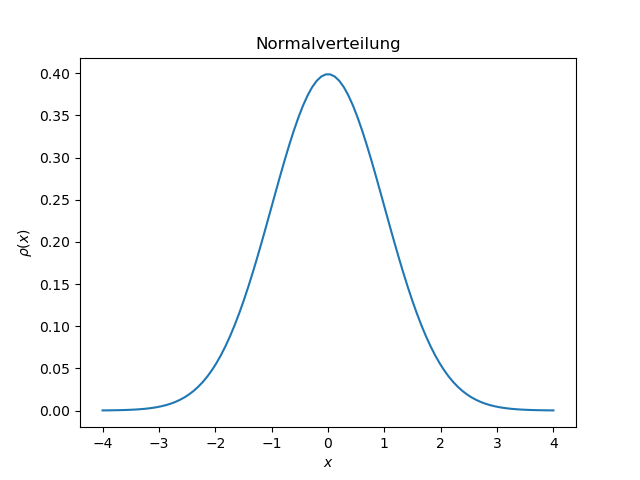
\includegraphics[width=.5\linewidth]{./gfx/gaussDistribution}
	\captionof{figure}{Die Normalverteilung}
\end{center}
\end{hintbox}

Wir erhalten einen Zufallsgenerator von NumPy über die Funktion \texttt{Generator} aus den bereitgestellten Konstruktoren:
\begin{codebox}[Zufallsgenerator explizit vorbereiten]
\begin{minted}[linenos]{python3}
from numpy import random
import time

seed = time.time()

rng = random.Generator(random.MT19937(seed))

print( rng.uniform() )    # Erzeugt eine zufällige Zahl zwischen 0 und 1
\end{minted}
\end{codebox}

Dieses Vorgehen mag Ihnen unnötig aufwändig erscheinen. Für den -- von den EntwicklerInnen von NumPy empfohlenen -- Generator PGC64 ist das Generator-Objekt schon vorbereitet und kann über \emph{Funktionen} von NumPy direkt angesprochen werden:

\begin{codebox}[Standard-Zufallsgenerator verwenden]
\begin{minted}[linenos]{python3}
from numpy import random
print( random.uniform() )    # Erzeugt eine zufällige Zahl zwischen 0 und 1
\end{minted}
\end{codebox}

Im Weiteren wird von Funktionen des Moduls \texttt{numpy.random} gesprochen. Behalten Sie aber auch im Kopf, dass (wo nichts gegenteiliges gesagt wird) ebenso auch Methoden mit gleichem Namen und Verhalten existieren, die auf solchen explizit gewählten Zufallsgeneratoren aufsetzen.

\subsection{Verteilungen}
Auf die Feinheiten der Stochastik kann hier leider nicht näher eingegangen werden. Stattdessen sollen die wichtigsten Verteilungen mit einigen nützlichen Eigenschaften vorgestellt werden. Eine Übersicht aller von NumPy bereitgestellten Distributionen samt ausführlicher Beschreibung finden Sie unter \url{https://numpy.org/doc/stable/reference/random/generator.html#distributions}.

Die Funktion \texttt{random} erzeugt gleichverteilte Zufallszahlen im Intervall $[0, 1)$, also zwischen 0 (eingeschlossen) und 1 (ausgeschlossen). Ausgegeben wird diese Zahl als \inPy{float}. Optional kann auch der Parameter \texttt{size} übergeben werden, um ein NumPy-Array zu erzeugen. \texttt{size} kann dabei entweder ein \inPy{int} sein, und beschreibt dann die Länge eines eindimensionalen NumPy-Arrays, oder ein \inPy{tuple}, der die Ausmaße des mehrdimensionalen Arrays in jeder Richtung beschreibt. Jeder Eintrag des Arrays wird dabei neu gezogen:

\begin{tcbraster}[raster columns=2,
                  raster equal height,
                  nobeforeafter,
                  raster column skip=0.5cm]
\begin{codebox}[Beispiel: \texttt{random}]
\begin{minted}[linenos]{python3}
from numpy import random
print( random.random() )
print( random.random(3) )
print( random.random((3, 3)) )
\end{minted}
\end{codebox}
%
\begin{cmdbox}[Ausgabe: \texttt{random}]
\begin{minted}{text}
0.7451593799574697
[0.74561109 0.85833608 0.00708435]
[[0.08326234 0.05691519 0.52119071]
 [0.39721293 0.18348375 0.29456297]
 [0.19200617 0.93908539 0.88486547]]
\end{minted}
\end{cmdbox}
\end{tcbraster}
Das Verhalten des optionalen Parameters \texttt{size} gilt in dieser Form auch für alle anderen Funktionen, die von \texttt{numpy.random} zur Verfügung gestellt werden.

Werden nur Ganzzahlen benötigt, so können diese über die Funktion \texttt{randint} bzw. die Methode \texttt{integers} erzeugt werden. Erwartet werden die Parameter \texttt{low} und \texttt{high}; optional kann auch \texttt{size} übergeben werden. Erzeugt werden so Ganzzahlen im Intervall [\texttt{low}, \texttt{high}). Für Fließkommazahlen zwischen vorgegebenen Grenzen kann in gleicher Art \texttt{uniform} benutzt werden: 

\begin{tcbraster}[raster columns=2,
                  raster equal height,
                  nobeforeafter,
                  raster column skip=0.5cm]
\begin{codebox}[Beispiel: \texttt{uniform} und \texttt{randint}]
\begin{minted}[linenos]{python3}
print(random.uniform(2, 5, size=3))
print(random.randint(2, 5, size=3))
\end{minted}
\end{codebox}
%
\begin{cmdbox}[Ausgabe: \texttt{uniform} und \texttt{randint}]
\begin{minted}{text}
[3.23220015 4.14602223 3.11928896]
[4 2 4]
\end{minted}
\end{cmdbox}
\end{tcbraster}

\begin{minipage}[T]{.65\linewidth}
\setlength{\parskip}{\medskipamount}
Die meisten Verteilungen haben zwei Parameter \texttt{loc} und \texttt{scale}. Dabei beschreibt \texttt{loc} den \emph{Lageparameter} (meist der Erwartungswert oder der häufigste Wert der Verteilung; bei symmetrischen Verteilungen ist dies derselbe Wert) und \texttt{scale}, wie \enquote{eng} die Verteilung ist, \ie wie groß die Streuung ist.

In Abb. \ref{fig:LaplaceDist} beispielsweise ist die Laplace-Verteilung um den gemeinsamen Erwartungswert $0$ aber mit verschiedenen Streuungen $\sigma$ aufgezeichnet.
Siehe auch \url{https://de.wikipedia.org/wiki/Laplace-Verteilung} für Details zur Laplace-Verteilung.

Die Funktionen \texttt{normal} und \texttt{laplace} folgen diesem Schema. Sie erzeugen jeweils eine um \texttt{loc} zentrierte Normal- bzw. Laplace-Verteilung mit Streuung \texttt{scale}.
\end{minipage}
%
\hspace{1em}
%
\begin{minipage}[T]{.3\linewidth}
	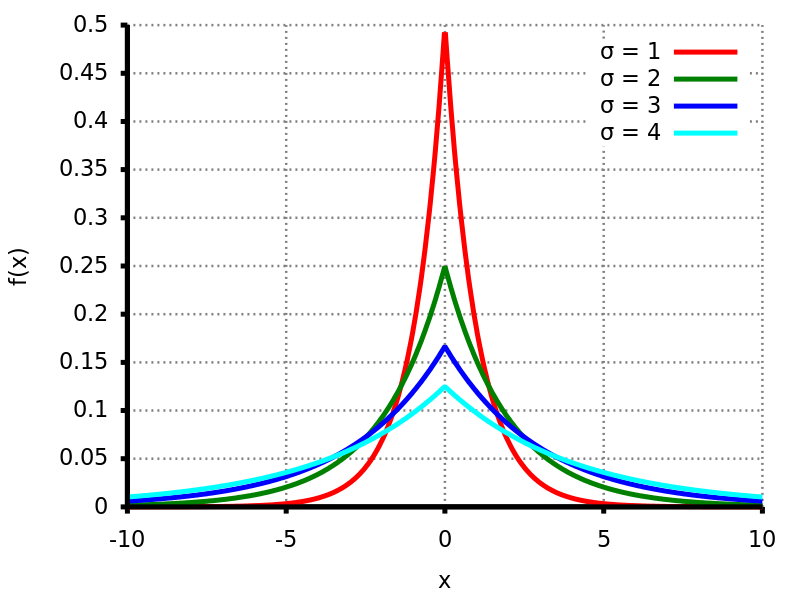
\includegraphics[width=\linewidth]{./gfx/LaplaceDistribution}
	\captionof{figure}{Laplace-Verteilung mit verschiedenen Streuungen $\sigma$}
	\label{fig:LaplaceDist}
\end{minipage}

\begin{codebox}[Beispiel: \texttt{normal} und \texttt{laplace}]
\begin{minted}[linenos]{python3}
from numpy import random
import matplotlib.pyplot as plt

dataGauss   = random.normal (0,  1 , size=50000)
dataLaplace = random.laplace(0, 0.3, size=50000)

fig = plt.figure()
drw = fig.add_subplot()

drw.hist(dataGauss  , bins=100, histtype='step', label='normal distribution')
drw.hist(dataLaplace, bins=100, histtype='step', label='Laplace distribution')
drw.legend()

plt.show()
\end{minted}
\end{codebox}

\begin{tcolorbox}[title=Ausgabe: \texttt{normal} und \texttt{laplace}]
\begin{center}
	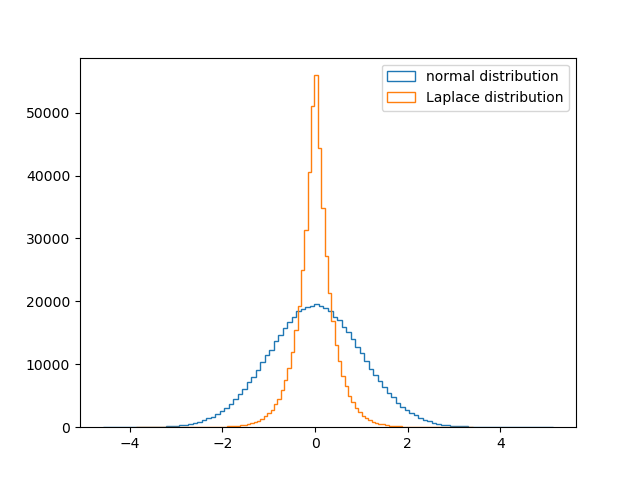
\includegraphics[width=.6\linewidth]{./gfx/gaussVsLaplace}
	\captionof{figure}{Histogramme von Zufallszahlen mit Normal- und Laplace-Verteilung}
\end{center}
\end{tcolorbox}

\subsection{Weitere Funktionen}
Schließlich kann \texttt{choice} genutzt werden, um zufällige Elemente aus einem Array auszuwählen. Die Wahrscheinlichkeit für jedes Element ist hier gleich.

\texttt{shuffle} kann genutzt werden, um ein bestehendes Array zu durchmischen. Mit \texttt{permutation} kann eine durchmischte Kopie eines Arrays erstellt werden, ohne die Originaldaten zu verändern.

\begin{tcbraster}[raster columns=2,
                  raster equal height,
                  nobeforeafter,
                  raster column skip=0.5cm]
\begin{codebox}[Beispiel: \texttt{uniform} und \texttt{randint}]
\begin{minted}[linenos]{python3}
import numpy as np
from numpy import random

A = np.arange(20).reshape(4, 5)
B = random.permutation(A)

print(A)
print(B)

random.shuffle(A)
print(A)
\end{minted}
\end{codebox}
%
\begin{cmdbox}[Ausgabe: \texttt{uniform} und \texttt{randint}]
\begin{minted}{text}
[[ 0  1  2  3  4]
 [ 5  6  7  8  9]
 [10 11 12 13 14]
 [15 16 17 18 19]]
[[10 11 12 13 14]
 [ 0  1  2  3  4]
 [ 5  6  7  8  9]
 [15 16 17 18 19]]
[[ 5  6  7  8  9]
 [15 16 17 18 19]
 [ 0  1  2  3  4]
 [10 11 12 13 14]]
\end{minted}
\end{cmdbox}
\end{tcbraster}
